\documentclass[11pt]{article}

\usepackage{epsfig}
\usepackage{fullpage}

\def\not{\mbox{${\tt '\backslash+'/1}$}}

\newcommand{\version}{Version 2.1}

\newcommand{\demo}[1]{\hspace*{1.5cm}{\sf #1}}
\newcommand{\desc}[1]{\item[{\tt #1}]\hspace*{1mm}\newline}

\begin{document}

\thispagestyle{empty}
\title
          {XSB \version \\ Technical Reference Manual}

\author{     Konstantinos Sagonas \\ Terrance Swift \\ Jiyang Xu
}
\maketitle

\newpage

\section*{	 	Credits	and Acknowledgments		 }
%			===========================

SB-Prolog was initially developed at the State University of New York
at Stony Brook, and at the University of Arizona.

A version of SB-Prolog was later developed at ECRC by Jiyang Xu and
called PSB-Prolog.  XSB is based on PSB-Prolog, and provides support
for many extensions to Prolog: among them tabling and HiLog.

This draft version of the technical reference manual is intended to
document features which are common to both systems.  Most of the
material in Section~\ref{sec:compiler} was written by Kostis Sagonas.
Sections~\ref{sec:comp-emu}--\ref{sec:libs} were written long ago by
Jiyand Xu and not seriously updated ever since --- rely upon them at
your own risk!  Section~\ref{sec:tabling} was written by Terry Swift.
The remaining sections were written more or less by all authors of
this technical manual.

Fuller credits can be fount in the {\it The XSB Programmer's Manual}.
\newpage

\tableofcontents

\newpage

\listoftables

\newpage

\listoffigures

\newpage

\section                 {Introduction}
%                        ==============


Novice users should first read the companion document ``{\it The XSB
Programmer's manual}'' before reading further.

XSB is still under development at the time of this writing, and
this documentation attempts to reflect the current status of the system.


\section{Compiler} \label{sec:compiler}
%======================================

The compiler of XSB is written in (XSB)-Prolog. It transforms
a source program module into an object code (byte code) module.
We begin by presenting the various phases of the compilation
process, the major modules of the compiler and their functionality
(in approximate order of use) and we finally describe the various
data structures that the modules of the compiler operate on.

\subsection{The Compilation Process and its Phases}
%==================================================
The compiler accomplishes the compilation process roughly in the
following three major phases:
\begin{enumerate}
\item	Module (global) level compilation phase.
\item	Predicate level compilation phase.
\item	Clause level compilation phase.
\end{enumerate}

Each of these phases is further divided in steps (subphases) 
which we describe in detail below.

\subsubsection{Module level compilation phase}
%---------------------------------------------
The module level compilation phase is the front-end of the XSB
compiler, where various global analyses and compilation techniques
take place.  All steps of this phase operate on the module as a whole
(encoded in the {\it internal source form} that is introduced later).
The following list describes possible steps of this phase.  We note
that some of the described steps are currently not implemented but their
position in the following list reflects various dependencies between them.
\begin{description}
\item[parsing]
	Reads in the source program files (in {\it external source form})
	and stores the information in the {\it internal source form}.
	A symbol table is included in the internal source form.
\item[use inference]
	Performs necessary inference such as detecting undefined predicates,
	implicit exported/global/local symbols, symbols that are never
	used, etc.  This step should return the list of exported
	predicates (symbols) of the module, so that they are used in
	the following steps.
\item[mode inference]
	Performs mode inference, annotating predicates with mode declarations
	(pragmatic information).  This step is currently not implemented,
	but should be of considerable use in (some of) the following steps.
\item[call specialisation]
	Specialises predicates according to (partially instantiated)
	call patterns that appear in the module.  One instance of this
	specialisation is for HiLog predicates.
\item[table declaration]
	Provided that the {\tt auto\_table} option of the compiler is
	on, this step automatically chooses a subset of predicates that
	should be tabled so that all possible cycles that cannot be proven
	terminating contain at least one tabled predicate.  This step
	currently employs a very simple termination checker to infer
	termination proofs for immediately recursive predicates for which
	mode information is known.
	A related step with the declaration of tabled predicates is a step
	that checks for semantic violations in the use of tabling
	(i.e. uses of cuts or nots across tabled predicates).
\end{description}
By the end of the module level compilation phase, the symbol table
should be complete and it could be dumped into the byte code and the
optional assembly file.  All symbols introduced by the following
phases should be {\em internal\/} to the module under compilation.

\subsubsection{Predicate level compilation phase}
%------------------------------------------------
The various steps in this phase share the property that they operate
on individual predicates, rather than on the whole module.  Some of
the operations performed in this phase, however, may produce a
predicate block (set of related predicates) out of a single predicate. 
\begin{description}
\item[cut transformation]
	Mimics a source-level transformation that cut-transforms predicates
	that contain cuts, nots and conditional statements.
\item[transformational indexing]
	Performs transformational indexing (unification factoring).
\item[index]
	Generates indexing instructions in {\it internal byte code
	form}, the Prolog representation of byte code (XWAM instructions).
\item[clause compilation]
	Performs the clause level compilation phase, returning a list of
	XWAM instructions in internal byte code form.
\item[peephole optimisation]
	Performs peephole optimisation on the internal byte code form.
\item[assemble]
	If the compiler option {\tt dumpasm} is on, outputs the byte code
	to the assembly file, in the {\it assembly form}.
\item[object code generation]
	Converts the internal byte code form into {\it byte code form} which 
	is written into the object file.
\end{description}

\subsubsection{Clause level compilation phase}
%---------------------------------------------
This phase is essentially the back-end of the XSB compiler and its
purpose is to generate (optimal) XWAM code for each clause.  The
substeps of this phase are (very roughly) the following:
\begin{description}
\item[clause flattening]
	Flattens each clause so that no nested structures occur in it.
\item[clause processing]
	Transforms each clause into an {\it intermediate form}, where
	pragmatic information for its variables is collected.
\item[XWAM code generation]
	Translates the intermediate form into the {\it internal byte 
	code form}.
\end{description}

As we have seen, a Prolog program can be in following forms:
\begin{itemize}
\item	external source form, (usually in {\tt *.P} and {\tt *.H} files);
\item	internal source form;
\item	intermediate form;
\item	internal byte code form;
\item	assembly form, in {\tt *.A} files;
\item	byte code, in {\tt *.O} files.
\end{itemize}
Finally, there is yet another form:
\begin{itemize}
\item	memory form, the memory image after loading.
\end{itemize}


\subsection{Compiler modules and their functionality}
%====================================================
\begin{description}
\item[compile.P] The top-level driver of the compiler.
\item[parse.P]	Uses Prolog's built-in predicate {\tt read/2} to parse
		the source module and performs initial symbol table registry.
		Uses {\bf singleton.P} to check for singleton variables in
		clauses, and the methods of {\bf symtab.P} (the symbol table
		manipulation module).
\item[useinfer.P]
		Performs inference of exported predicates/structures/constants
		marking them as exported/local/global.  It also prints out
		warnings for unused/undefined predicates.
\item[spec.P]	Specialises predicates according to partially instantiated
		call patterns that appear in the module.  One instance of this
		specialisation is for calls to HiLog predicates.  Calls to
		these predicates are usually partially instantiated.
\item[tabdef.P] Builds the call graph for the module and automatically chooses
		a subset of predicates that will be tabled.
\item[cutcheck.P]
		Checks for semantic violations in the use of cuts,
		if-then-elses, or nots in combination with tabled predicates.
\item[preprocess.P]
		Preprocesses predicate definitions that contain cuts, nots,
		or conditional statements.  It essentially performs
		a source to source cut transformation.  It uses the
		following module:
	\begin{description}
	\item[pre\_cond.P] Handles conditional statements (with inline tests)
		that need no choice points.  Currently, it is limited to
		branches of a disjunction with mutually exclusive inline
		tests, e.g. {\tt '>='/2} and {\tt '<'/2} with the same
		arguments.
	\end{description}
\item[tp\_index.P] Indexes a predicate, generating {\tt try/retry/trust}
		and {\tt switchon*} instructions for the predicate's clauses.
\item[tprog.P]	Translates clauses into XWAM code.  It is the ``heart''
		of the clause-level compilation phase. Calls in approximately
		the following order:
	\begin{description}
	\item[flatten.P] Flattens out structures in clauses along the lines of
		{\tt p(f(g(D))) => p(f(Y)),Y = g(D)}.  The code in that module 
		is much more general since it can flatten to any level by
		simply redefining the predicate {\tt level\_allowed/1}.
	\item[inprog.P] Transforms a clause in internal source form into the
		intermediate form, collecting pragmatic information
		about the clause.
	\item[varproc.P] Processes the variables of the clause collecting
		pragmatic information about their occurrences.
	\item[tp\_geninline.P] Generates code for inline predicates.
	\item[tp\_cond.P] Generates special code for conditionals with
		inline test parts.  Uses {\bf tp\_comp.P} and {\bf
		tp\_eval.P}.
	\item[tp\_goal.P] Generates {\tt get*/put*/bld*/uni*} XWAM instructions
 		for each goal (including the head).  Uses {\bf tp\_var.P}.
	\item[tp\_eval.P] Generates code for arithmetic expressions.
	\end{description}
\item[peephole.P]
		Performs peephole optimisation for one predicate at a time.
\item[asm.P, asm\_pass2.P]
		Generates XWAM byte code from internal byte code
		representation.  Use information in the instruction table 
		found in module {\bf asm\_inst.P}.
\item[asm\_opt.P] Further optimises the byte code for a predicate block
		by changing some {\tt call} and {\tt excute} XWAM instructions
		to {\tt calld} and {\tt executed} instructions respectively.
\end{description}

\subsection{Internal Source Form}
%================================

The internal source form is represented by the following Prolog data structure:

\demo{    Module = module(SymTab, DcList, ClList, QrList) }

{\sf SymTab} is the symbol table. Because of the complexity of its
structure, and the fact that the symbol entry is also used in
several other program forms, its form will be introduced in the
next subsection.

{\sf DcList} is currently not used, but it might be used for storing
directives found in the module, so that they can be easily dumped out.

{\sf ClList} represents the normal clauses and is a list of:

\demo{   pred(Symbol, [Clause1, Clause2, \ldots, ClauseN], Pragma)        }

which represents all the clauses of the predicate {\tt Symbol}
(a symbol table entry, see next subsection).

Each {\sf Clause} has the form:

\demo{	clause(Arguments, Body, Pragma)				}

where {\sf Arguments} is a list of {\tt Term}s (see below) and {\sf Body}
is a {\tt Goal} which can be one of the following:

\begin{description}
\desc{and(Goal1, Goal2)}
	Represents a conjunction of two goals {\tt Goal1} and {\tt Goal2}.
\desc{or(Goal1, Goal2)}
	Represents a disjunction of two goals {\tt Goal1} and {\tt Goal2}.
\desc{if(Goal1, Goal2)}
	Represents the conditional execution of {\tt Goal2} provided
	that {\tt Goal1} succeeds.
\desc{not(Goal)}
	Represents the {\em compiled} negation of a {\tt Goal}.
 	For maximal developer's confusion, compiled negations are calls
	to the standard predicates \not\ and {\tt fail\_if/1}, but not
	to the {\tt not/1} standard predicate.
\desc{goal(Symbol, Arguments)}
	{\tt Symbol} is a symbol table entry representing the predicate
	symbol of the atomic goal, and {\tt Arguments} is a list of
	{\tt Term}s.
\desc{inlinegoal(Name, Arity, Arguments)}
	Represents an atomic goal whose predicate, {\tt Name/Arity},
	is a predicate that is expanded inline when compiled;
	{\tt Arguments} is a list of {\tt Term}s, representing the
	arguments of the goal.  The inline predicates of XSB are given
	in table~\ref{inlinepredicatetable}.
\end{description}

\begin{table}[htbp]\centering{\tt
\begin{tabular}{lllll}
\verb|'='/2|	&\verb|'<'/2|	&\verb|'=<'/2|	&\verb|'>='/2| &\verb|'>'/2| \\
\verb|'=:='/2|	&\verb|'=\='/2|	&is/2		&\verb|'@<'/2| &\verb|'@=<'/2|\\
\verb|'@>'/2|	&\verb|'@>='/2|	&\verb|'=='/2|	&\verb|'\=='/2|&fail/0 \\
true/0		&var/1		&nonvar/1	&halt/0        &'!'/0 \\
'\_\$cutto'/1	&'\_\$savecp'/1	&'\_\$builtin'/1
\end{tabular}}
\caption{The Inline Predicates of XSB}\label{inlinepredicatetable}
\end{table}

A {\tt Term} can be one of the following:

\begin{description}
\desc{varocc(Vid)}
	A variable; {\tt Vid} is an integer or a constant that identifies
	the variable.  Different variables of the same clause have distinct
	identifiers.  The XSB parser assigns integers as variable identifiers,
	while modules like {\tt spec} and {\tt preprocess} assign atoms of
	the forms {\tt '\_v\#'} as variable identifiers.
\desc{constant(Symbol)}
	A constant symbol represented by the symbol table entry {\tt Symbol}.
\desc{integer(Int)}
	An integer having value {\tt Int}.
\desc{real(Real)}
	A floating number having value {\tt Real}.
\desc{structure(Symbol, Arguments)}
	A structure whose primary functor is {\tt Symbol} and whose
	arguments are elements in the list {\tt Arguments}.
\end{description}

{\sf QrList} represents queries (commands) of the module and has the
same form as {\sf ClList} except that it contains only one predicate
definition, and the predicate has the system supplied name \verb+'_$main'/0+.
%$

\subsection{Symbol Table Format}
%===============================

The symbol table is implemented as an {\em abstract data type} by the
module {\tt symtab}.

Abstractly, the symbol table is a table of symbols. A symbol
is an abstract object that {\em can be accessed only by the methods
(interface routines)} introduced later.  It is considered a bad
programming habit to access the symbol table by any other means. 
The structure of the table and symbols are hidden from the users
of the module.  To put more emphasis on our argument, we avoid
presenting the internal structure of the symbol table and we only
do so for the symbol table entries.

\subsubsection{Internal structure of the entries}
%------------------------------------------------

Each symbol table entry is internally represented as:

\demo{		sym(Name, Arity, Properties, Index)		}

where {\sf Properties} has the form:

\demo{     prop(Category, Scope, Defined, Used, EP, PragmaList)	}

{\sf Category} is either undetermined (free variable) or one of the
category properties.  {\sf Scope} is one of the scope properties.
{\sf Defined} is either {\tt defined} or {\tt undef}. 
Similarly {\sf Used} is either {\tt used} or {\tt unused}.
{\sf EP} is {\tt ep(Offset)}, and finally {\sf PragmaList} is a
list of other pragma properties.  All of these are described below.

\subsubsection{Symbol properties}
%--------------------------------
As mentioned, each symbol has a {\sf Name} attribute and an {\sf Arity}
attribute that can be accessed through methods.  A symbol is
also associated with a unique ordinal number called {\sf Index} that
represents the location of the symbol in the output assembly and
object files.  In addition, a symbol can have one or more of the
following optional attributes called {\sf Properties}:

\begin{enumerate}
\item	Category (or type) of the symbol (a symbol can have at most one
	property in this group). This attribute tells the type of usage
	of the symbols, namely, as a predicate symbol, a module name, etc.
	\begin{description}
	\item[{\tt pred}]	The symbol is a predicate.
	\item[{\tt module}]	The symbol is a module name.
	\item[{\tt dynamic}]	The symbol is a dynamic predicate, currently
				not used (though it should be).
	\end{description}
	Such information will be passed into byte code files and then to the
	emulator when the files are loaded. See Table \ref{t:symcat} on page
	\pageref{t:symcat} for the corresponding categories of symbols
	in the emulator.

\item	Scope.  A symbol can have at most one property in this group,
	and this is ensured by the {\tt sym\_propin/2} method described below.
	\begin{description}
	\item[{\tt ex}]		The symbol is exported by this module.
	\item[{\tt im(Module)}]	The symbol is imported from the module
				{\tt Module}.
	\item[{\tt global}]	A global symbol that can be accessed
				(is visible) by any module.
	\item[{\tt local}]	The symbol is local to the module.
	\item[{\tt internal}]	The symbol is generated internally
				during compilation.
	\end{description}
\item	Defined checking.  The following properties are only used during usage 
	checking, and have meaning only for predicate symbols.
	\begin{description}
	\item[{\tt defined}]	The symbol is a predicate that is defined in
				this module.
	\item[{\tt undef}]	A predicate symbol that is not defined in
				this module, or imported from another module.
	\end{description}
\item	Usage checking.  The following properties are only used during usage 
	checking, but are applicable to all symbols.
	\begin{description}
	\item[{\tt used}]	A symbol that is used by some predicate
				definitions in this module.
	\item[{\tt unused}]	A symbol that is not {\tt used}.
	\end{description}
\item	Entry point of predicate (used by the assembler):
	\begin{description}
	\item[{\tt ep(Location)}]
		{\tt Location} is an offset of the starting point of the
		code to the beginning of the entire text segment.
	\end{description}
\item	Pragmatic information
	\begin{description}
	\item[{\tt index(Position)}]
		Indicates the fact that the predicate will be indexed on
		its {\tt Position}-th argument.  The default position is 1.
	\item[{\tt tabled(Tabind,Arity)}]
		Used for tabled predicates.  {\tt Tabind} is the table
		identification number and {\tt Arity} is the arity of
		the predicate symbol.
	\item[{\tt mode(p(+,.,?,..,-))}]
		Indicates mode usage of the predicate {\tt p/N}.  A predicate
		can have several different instances of this information.
	\end{description}
\end{enumerate}


\subsubsection{Methods for accessing the Symbol Table}
%-----------------------------------------------------
The following are all the methods implemented:

\begin{description}
\desc{sym\_insert(+Name, +Arity, +PropList, $\pm$SymTab, -Sym)}
	Inserts a symbol with name {\tt Name} and arity {\tt Arity} into 
	the symbol table {\tt SymTab}, and returns the symbol entry (the
	abstract object) in {\tt Sym}.  {\tt PropList} is a list of
	properties that are associated with the symbol.  If the symbol
	already exists in the symbol table, only the properties are
	added, and the symbol entry is returned.
\desc{sym\_count(+SymTab, -Number\_of\_Entries)}
	Returns the number of symbol entries in the symbol table.
\desc{sym\_scan(-Sym, +SymTab, -SymTabRest)}
	Gets an (arbitrary) symbol entry {\tt Sym} from the symbol table 
	{\tt SymTab}, and returns the rest of the symbol table in 
	{\tt SymTabRest}.  This procedure can be used to obtain
	all the symbols through backtracking, though we recommend the
	use of the more efficient {\tt sym\_gen/2} method, below.
\desc{sym\_gen(-Sym, +SymTab)}
	Gets an (arbitrary) symbol entry {\tt Sym} from the symbol table 
	{\tt SymTab}.  Best used to generate all symbols through
	backtracking.
\desc{sym\_empty(+SymTab)}
	Succeeds iff the symbol table is empty.
\desc{sym\_propin(+PropList, +Sym)}
	Inserts a list of additional properties into the symbol table
	entry, while checking for errors (inconsistencies).
	{\tt PropList} can either be a list or a single property.
\desc{sym\_prop(+Prop, +Sym)}
	Succeeds when the symbol table entry {\tt Sym} possesses the
	given property.
\desc{extract\_symlist(+Prop, -SymList, +SymTab)}
	{\tt Prop} is a single or a list of properties.
	The predicate returns a list of symbols ({\tt SymList}) that
	have the property {\tt Prop} (or have all the properties listed
	in {\tt Prop}).
\desc{sym\_name(+Sym, -Name, -Arity)}
	Returns the name and the arity of the symbol.
\desc{sym\_offset(+Sym, -Index)}
	Returns the index number of the symbol.
\desc{sym\_category(+Sym, -Category)}
	Returns the category of the symbol.
\desc{sym\_env(+Sym, -Scope)}
	Returns the scope of the symbol.
\desc{sym\_type(+Sym, -Tabled)}
	Returns the tabled properties of the symbol, or alternatively
	succeeds iff the symbol is a tabled predicate symbol.
\desc{sort\_by\_index(+SymTab, -Sorted\_SymList)}
	Sorts the symbols in the symbol table {\tt SymTab} based on their
	index field, returning them in the list {\tt Sorted\_SymList}.
\desc{sym\_complete($\pm$SymTab)}
	Completes the symbol table.
\end{description}



\subsection{Intermediate Program Form}
%=====================================

The intermediate program form is generated mainly by the {\tt
preprocess} module that performs cut and not transformations, and by
the predicate {\tt inprog/2} (in module {\tt inprog}).  The intermediate
program form is only used in the last two phases of the compiler.
After the gradual evolution of the XSB compiler, the intermediate program
form is not much different from the internal source form, except
pragma information being added to variable occurrences.  Also, {\tt if}
and {\tt not} constructs are changed by the cut-transformation.

The form of predicates is the same as the one of the internal source
form, while each {\tt Clause} has the form

\demo{	clause(Arguments, Body, CPrag)				}

where {\sf Arguments} is a list of {\tt Term}s (see below), {\sf CPrag}
is a clause-pragma structure (whose form will given later), and
{\sf Body} is a {\tt Goal} which can be one of the following:

\begin{description}
\desc{nil}
	An empty body.  Used when the clause is a fact that needs no
	flattening.
\desc{and(Goal1, Goal2)}
	Represents a conjunction of two goals {\tt Goal1} and {\tt Goal2}.
\desc{or(Goal1, Goal2)}
	Represents a disjunction of two goals {\tt Goal1} and {\tt Goal2}.
\desc{if\_then\_else(TestGoal, TrueGoal, FalseGoal)}
	Represents an if-then-else construct (maybe constructed by analysis),
	in which {\tt TestGoal} is a goal that contains only inline tests,
	while {\tt TrueGoal} and {\tt FalseGoal} are {\tt Goal}s.
\desc{goal(Symbol, Arguments)}
	{\tt Symbol} is a symbol table entry representing the predicate
	symbol of the atomic goal, and {\tt Arguments} is a list of
	{\tt Term}s.
\desc{inlinegoal(Name, Arity, Arguments)}
	Represents an atomic goal whose predicate is a predicate
	{\tt Name/Arity} that is expanded inline when compiled;
	{\tt Arguments} is a list of {\tt Term}s, representing the
	arguments of the goal.
\end{description}

A {\tt Term} can be one of the following:

\begin{description}
\desc{varocc(Vid, VPrag)}
	A variable; {\tt Vid} is an integer or a constant that identifies
	the variable. Different variables of the same clause have distinct ids.
	{\tt VPrag} is a variable-pragma structure whose form is given below.
\desc{constant(Symbol)}
	A constant symbol represented by the symbol table entry {\tt Symbol}.
\desc{integer(Int)}
	An integer having value {\tt Int}.
\desc{real(Real)}
	A floating number having value {\tt Real}.
\desc{structure(Symbol, Arguments)}
	A structure whose primary functor is {\tt Symbol} and whose
	arguments are elements in the list {\tt Arguments}.
\end{description}

The variable-pragma structure is now implemented by an abstract datatype.
The attributes and their accessing methods are given in Table~\ref{t:vprag}.

\begin{table}\centering
\begin{tabular}{|l|l|l|}
\hline
Attribute	& Value			& Access method			\\
\hline \hline
{\sf type}	& {\tt p} - permanent	& vprag\_type(VPrag, Type)	\\
		& {\tt t} - temporary	&				\\
		& {\tt vh} - void head	&				\\
{\sf location}	& an integer		& vprag\_loc(VPrag, Loc)	\\
{\sf use}	& see below		& vprag\_use(VPrag, Use)	\\
{\sf nouse}	& see below		& vprag\_nouse(VPrag, NoUse)	\\
\hline
{\sf context}	& {\tt h} - head	& vprag\_context(VPrag, Context)\\
		& {\tt i} - inline goal &				\\
		& {\tt b} - other goal	&				\\
{\sf level}	& {\tt t} - top	level	& vprag\_level(VPrag, Level)	\\
		& {\tt s} - second level&				\\
{\sf argument
     position}	& an integer		& vprag\_argno(VPrag, Argno)	\\
{\sf occurrence}& {\tt f} - first	& vprag\_occ(VPrag, Occ)	\\
		& {\tt l} - last	& 				\\
		& {\tt v} - void	& 				\\
		& {\tt s} - other	& 				\\
{\sf in last
     chunk}	& {\tt 1} - yes		& vprag\_lastchunk(VPrag, Yes)	\\
		& {\tt 0} - no		&				\\
\hline
{\sf type1}	& see below		& vprag\_type1(VPrag, Type)     \\
\hline
\end{tabular}
\caption{Variable Pragma Access Methods}
\label{t:vprag}
\end{table}

The attributes {\sf type, location, use} and {\sf nouse} are shared
by all occurrences of the same variable, while the other attributes
depend on the specific occurrence.

For temporary variables, the {\sf location} attribute records the
register number, while for permanent variables it is the offset in
the activation record (the first variable has offset 2).

For temporary variables, the {\sf use} attribute stores a list of
integers that represent the register numbers the variable is preferred
to be allocated, and the {\sf nouse} attribute stores a list of 
registers that the variable should not be allocated.

For permanent variables, occurrences in the last chunk may be
{\it unsafe} (first occurrence of a variable that does not appear in
the head), or may need to be {\it dereferenced} (all subsequent
occurrences).  This information is stored in the {\sf use} attribute
as {\tt u} and {\tt d} respectively, or {\tt p} when neither case
applies (variables that appear in the head).  The attribute
{\sf type1} is a derived attribute that is the same as the attribute
{\sf type} except when the variable is permanent and occurs in the
last chunk, in which case {\sf type1} is the same as the {\sf use}
attribute.  {\sf nouse} attributes are not used for permanent
variables.

The internal structure of variable-pragmas has the form:

\demo{	vrec(Context,Level,Argno,Occ,v(Type,Loc,Use,NoUse),LastChunk)	}

where the {\sf v(\ldots)} part is shared by all occurrences of
the variable.

The clause-pragma structure takes the following form

\demo{		crec(ARSize, Label)		}

where {\sf ARSize} is the size of the activation record, and {\sf Label}
is the label of the clause.

%and {\sf VarList} is a list of {\sf variable(Vid, VCPrag)}, one
%for each variable (not each occurrence).  {\sf VCPrag} is the shared
%portion of the variable-pragmas of all occurrences of the variable.


\subsection{Compiler Options}
%============================

Besides the compiler options introduced in the {\it XSB Programmer's Manual},
there are some other options that exist mainly for debugging and profiling
purposes.  Here is a list of compiler options.

\begin{itemize}
\item   Inference Options:
	\begin{description}
        \item[nocompile] Do not compile, but do inferencing only.
	\item[spec\_off] Do not perform specialisation of partially
			 instantiated calls.
        \item[modeinfer] Performs mode inferencing (currently not implemented).
	\end{description}
\item   Debugging Options:
	\begin{description}
        \item[verbo]	Prints out intermediate information during compiling.
        \item[dump\_asm] Generates a {\tt *.A} file.  Known to {\em not\/}
			work when predicates are cut-transformed.
	\item[dump\_spec] Generates a {\tt *.spec} file, containing the result
			of specialising partially instantiated calls to
			predicates defined in the module.  The result is in
			Prolog source code form.
	\item[dump\_ti] Generates a {\tt *.ti} file, containing the result
			of applying transformational indexing (unification
			factoring) to some subset of the predicates defined
			in the module.  The result is in Prolog source code
			form.
	\end{description}
\item   Pragma Options:
	\begin{description}
        \item[sysmod]	Mainly used for the compilation of system modules.
			Standard predicates are not assumed to be automatically
			imported, and the compiler does not generate warnings
			for the redefinition of standard predicates.
			Also, all primitive predicates are compiled inline
			(calling {\tt '\_\$builtin'/1}).  Because of that,
			there are some modules (like {\tt syslib/standard.P},
			or {\tt lib/setof.P}) that {\em must\/} be compiled
			with this option.
        \item[index\_off] The compilation phase will not generate indices.
	\end{description}
\end{itemize}





\section{Compiler-Emulator Interface} \label{sec:comp-emu}
%=========================================================

This section introduces the byte code and object file format, and
built-in predicates representations. Since the compiler and
the emulator must agree on these formats, we use an independent
section here to discuss them.

\subsection{WAM Instruction Format}
%==================================

All the abstract machine instructions
implemented by XSB \version \mbox{} are listed in Appendix A.


\subsection{Byte Code File Format}
%================================

A byte code file contains a data segment followed by several program
segments. Each segment is started by a magic number. The magic number
for the data segment (which is also the magic number for the whole
module) is 0x11121304 and the magic number for each program segment
is 0x11121306. Figure \ref{f:objectfile} gives an intuitive idea
what an object file looks like.

\begin{figure}
\begin{verbatim}
         ______________________
         |magic num 0x11121304|				Data segment
         -----------------------------------------
         |leng| module name (leng chars )        |  For basic module, leng = 0
         -----------------------------------------
         | psc count          |
         ----------------------
         ________________________________________________________________
         |Env |Cat |Arity|Len | ..... Name ....     |MLen| Mod name .....
         ----------------------------------------------------------------
           1    1     1    1        Len Bytes       | 1  |  MLen bytes
         ...                                         \-----------------/
         ...                                           when Env = im
         ...


         ______________________
      /  |magic num 0x11121306|                        A program segment
     /   -----------------------------------          in object code files
     |   |arity|leng| entry predicate name |
     |   -----------------------------------
     |   | text size (bytes)  |
     |   ----------------------
     |   | index size (bytes) |
   N |   ----------------------
     |
 times   --------------------------------------------
     |   | text subsegment ............
     |   ---------------------------------------------
     |   ----------------------------------------------
     \   | index subsegment ......................
      \  ----------------------------------------------

\end{verbatim}
\caption{Format of Object Code Files}
\label{f:objectfile}
\end{figure}

{\it Psc count} is the number of symbols in the data segment.  Each
symbol is represented by one byte {\it scope} (or environment --- {\tt
Env}), one byte {\it category} ({\tt Cat}), one byte {\it arity}, one
byte {\tt Leng} representing the length of the symbol's name, and
followed by the name string. If the symbol is imported from another
module, the name of that module follows further.

Categories and scopes are encoded into numbers in the byte code file.
Table \ref{t:symscope} lists the scopes, their codes and their symbolic
name used by the emulator.

\begin{table}\centering
\begin{tabular}{l|l|l|l}
\hline
Code & Name in compiler & Name in emulator & Comment		\\
\hline
   0 & ex	& T\_EXPORTED	& exported name			\\
   1 & local	& T\_LOCAL	& local name			\\
   2 & im(\_)	& T\_IMPORTED	& imported name			\\
   3 & imex	& T\_IMEX	& im/exported, not used now	\\
   4 & global	& T\_GLOBAL	& global name			\\
\hline
\end{tabular}
\caption{Scopes of Symbols}
\label{t:symscope}
\end{table}

The scope of a symbol is not stored in the memory after loading. See next
section for how they are processed during loading.

Table \ref{t:symcat} lists the categories, their codes and their symbolic
name used by the emulator.

\begin{table}\centering
\begin{tabular}{l|l|l|l}
\hline
Code & Name in compiler & Name in emulator & Comment		\\
\hline
  0 & ordinary	& T\_ORDI & unclassified name, may be changed to others \\
  1 & (dynamic)	& T\_DYNA & dynamic predicates, not used by the compiler \\
  2 & pred	& T\_PRED & predicate, including internal predicates	\\
  3 & (buffer)	& T\_PEXI & not used yet. Before, for globalset.	\\
  4 & module	& T\_MODU & module. Its emulator property is a psc-list \\
  5 & file	& T\_FILE & file. Its emulator property is a file number \\
  6 & (cons)	& T\_CONS & pure constant; not used			\\
  7 & (str)	& T\_STRU & pure structure symbol; not used		\\
  8 &		& T\_CSET & for conset/convalue, not used in C-code	\\
  9 & (string)	& T\_STRG & string; not used				\\
 10 &		& T\_RKEY & record key, not used in C-Code		\\
 11 &		& T\_ALIA & alias; its emulator property is a term	\\
 12 & (pred)	& T\_UDEF & unloaded predicate				\\
 13 & (foreign)	& T\_FORN & foreign predicate				\\
\hline
\end{tabular}
\caption{Symbol Categories}
\label{t:symcat}
\end{table}

The compiler currently only uses five categories: {\tt T\_ORDI,
T\_PRED, T\_MODU}, and {\tt T\_FILE}. The category {\tt T\_ORDI} is
indeed represented by a free variable rather than {\tt ordinary}
inside the compiler and is only filled in when writing into the byte
code file. The categories {\tt pred} and {\tt fun} are changed to {\tt
T\_UDEF} when writing into the byte code files.

The categories {\tt T\_CSET} and {\tt T\_RKEY} are used neither by the
compiler nor by the emulator, but are used by Prolog libraries.  {\tt
T\_DYNA} and {\tt T\_ALIA} are mainly used by Prolog libraries, but
the emulator is aware of them because special treatment is needed.
For the moment, T\_ALIA does not work for double word version of the
emulator. {\tt T\_FORN} is generated from a foreign language module.

{\tt T\_PEXI, T\_CONS, T\_STRU}, and {\tt T\_STRG} are not used
anywhere for now.

A program segment consists of a header, a text subsegment and an index
subsegment. The text subsegment is just a list of WAM instructions,
while the index subsegment consists of a number of blocks with the
following format:

\begin{verbatim}
                ---------------------------------------------
      cases     |247 |arit|      N1        |   N2           |
                ---------------------------------------------
             /  |ics |value           |   location     |
             |  ----------------------------------------
             |  | ln |location        |
             |  -----------------------
      N2     |      :
    arglabel |      :
             |      :
             |  ----------------------------------------
             \  |ics |value           |   location     |
                ----------------------------------------
\end{verbatim}

       247: op code for "cases"

       i,c,s,l,n: index on integer, constant, structure, list or nil

       N1: the order number of this index block; numbered
           from 1 (or 0?) up.

       N2: the number of cases (i.e. arglabels in the block)


\subsection{Byte Code File for Foreign Modules}
%==============================================

The byte code file for a foreign module contains only a data segment
(no program segments), and the foreign language object code is store
in the corresponding {\tt *.o} file. The magic number of a foreign module
is 0x11121308.  The header of the data segment has a slightly different
format from that of a normal byte code file. It contains one more entry
to store a string that is to be passed to the system loader ``ld'' when
the foreign code is dynamically loaded. The format of a foreign module
is shown in Figure \ref{f:formod}.

\begin{figure}
\begin{verbatim}
                +-----------------------+
                | magic num: 0x11121308 |
                +-----------------------+------------------+
                | len  |  module name (len size)           |
                +-----------------------+----------+-------+
                | len  |  "ld" option              |
                +-----------------------+----------+
                | psc count             |
                +-----------------------+

                +-----------------------+-------------------------------+
        count:  | 0   | 13  |arity|len  |  symbol name string           |
                +-----------------------+-------------------------------+
                ... ... ... ...
                ... ... ... ...
\end{verbatim}
\caption{Format of the byte code file for a foreign module}
\label{f:formod}
\end{figure}

\subsection{Assembly File Format}
%================================

\begin{verbatim}
        modname(Name).
        sym(P,A,PropList,'_').   \
        :                        |
        :                        |  Symbol Table
        :                        |
        sym(P,A,PropList,'_').   /
        ( code below )
\end{verbatim}


\subsection{Primitive Predicates}
%===============================

Primitive predicates (also called built-in predicates)
are predicates implemented directly by the emulator through the
WAM instruction 

\demo{		builtin(N)			}

where $N$ is the number assigned to the specific primitive predicate.

(Need to introduce internal data structures here!!!)

The symbolic names of the primitive predicates and their semantics
are introduced in the {\it User Manual}. Appendix B lists
their internal numbers.

These predicates are available when the module using them is compiled
with the option {\tt sysmod}, in which case they are translated
directly into WAM code. When you must use them in a module not compiled
with the option {\tt sysmod}, they have to be imported from a system 
module named {\tt machine}.




\section                 {The Emulator}
%                        ==============

This section mainly introduces those features of the emulator needed for
SLD.  Extensions for SLG will be covered later.

Besides the inference engine, the emulator mainly contains the following
data areas:

\begin{itemize}
  \item  A set of registers.
  \item  A set of flags.
  \item  A permanent space (mainly for programs and symbol tables).
  \item  A stack space which contains a global stack (or heap), a local stack,
     a trail stack, and a choice point stack.
\end{itemize}

\subsection{Emulator Versions}
%=============================

The structure of the XSB emulator is well organized into 
modules with as much abstraction as possible. This allows us to support
many different implementation techniques without modifying the code
significantly. The difference between the double word version
and the single word version, for instance, is only 3 type definitions
and about 25 simple macro definitions.

The following is a list of version options that you can set in the
emulator makefile (or source code).

\paragraph{Prolog data cell format. }
The memory unit for storing a Prolog term is called a {\it
data cell} or a {\it Prolog word}. Most Prolog implementations
use {\it single word} format, namely a Prolog word is implemented
with a single host machine word (of 32 bits). A few bits
of the word are used as tags, and the remaining bits are used
to store values. There are also Prolog implementations that use
{\it double word} format, namely a Prolog word is implemented
with two host machine words. One word is normally used to store 
value and the other is for tags and other usage.

XSB supports both a single word format and a double word
format.  In the single word version, 4 bits are used as tags, and the
remaining 28 bits are for all types of values. Integers are therefore coded only 
with 28 bits. Floating point values maintain double precision (64 bits) by default, 
but do so by being stored as single-word references to an internal structure that
contains the 64 bits of data. The double word version of XSB uses two host machine 
words (64 bits) as a Prolog word. One machine word is used for tag, and the other 
is for value. Integers and floating point numbers have the same format as the host
machine.

There is also a variation of the single word format, called {\it
one-and-half-word} or {\it single-word-by-reference}. 
The data cell format is the same as for the single word format,
but the identity of a data cell (the type {\tt Cell} in C) is the
reference (address) of it, rather than the data cell itself as in
the single word version. The double word version uses references
as data cell identities as well.

The selection of the data cell format is done by supplying 
in the {\it makefile} one of the variable definitions below:

\begin{verbatim}
        TAGOPTION = -DSW 	/* DSW is only option available for now */
        TAGOPTION = -DDW
        TAGOPTION = -DHW
\end{verbatim}

where {\tt SW} stands for single word format, {\tt DW} for double word
format, and {\tt HW} for one-and-half word format.

\paragraph{Debugging and testing modes. }
Another macro definition is used in the makefile
for generating a version for system debugging, or a version
for performance measurement, or for regular use.
Again, you must select exactly one of the three definitions below:

\begin{verbatim}
        DEBUGOPTION = -O
        DEBUGOPTION = -g -DDEBUG
        DEBUGOPTION = -PROFILE
\end{verbatim}

The {\tt PROFILE} option allows profiling of XWAM level instructions.


\paragraph{Other options. }

NOT\_RETURN\_HASHING will be a macro that will be used when returns are
not hashed but instead are kept in some other index structure.
Currently this macro has no effect, but other macros which will have
to be rewritten for alternate return indexing lie in the scope of this
ifdef.

The macro MMLARGE, calls load\_solution and save info as macros, rather
than as functions.  Its effect is minimal, however.

\subsection{Data Cell Format}
%============================

A data cell (Prolog word) contains a tag field and a value field.
Table \ref{t:datatags} lists all the tags used in XSB.
In single word format, the 4 least significant bits are used
as tags. Reference cell is an exception, in that the whole 32 bits
are used as the pointer (pure value), since the emulator ensures that
words are always aligned with four bytes boundary, the last two bits
are always 0. But the second last two bits cannot be used as normal tags.

\begin{table}\centering
\begin{tabular}{l|l|l|l}
\hline
Code	   & Name	& Explanation	    & Value			\\
\hline
0x0 (0000) & REF(FREE)	& reference	    & a pointer to another cell \\
0x1 (0001) & CS		& constant/structure& a pointer to a structure	\\
0x2 (0010) & INT	& integer	    & an integer		\\
0x3 (0011) & LIST	& list		    & a pointer to a pair	\\
0x4 (0100) & REF1	& refernence	    & a pointer to another cell \\
0x5 (0101) & STRING	& string	    & a pointer to the string	\\
0x6 (0110) & FLOAT	& floating number   & floating point number	\\
0x7 (0111) & (STRUCT)	& not used	    &				\\
0x8 (1000) & REF2	& reference	    & a pointer to another cell \\
0x9 (1001) &		& not used	    &				\\
0xa (1010) & INDEX	& indexed variable  & the index of the variable	\\ 
0xb (1011) &		& not used 	    &				\\
0xc (1100) & REF3	& reference	    & a pointer to another cell \\
0xd (1101) & (DELAY)	& not used 	    &				\\
0xe (1110) & DVAR	& not used	    &                           \\
0xf (1111) & (ESCAPE)	& not used	    &				\\
\hline
\end{tabular}
\caption{Data Cell Tags}
\label{t:datatags}
\end{table}


\subsection{Registers}
%=====================

Table \ref{t:register} lists the registers used by the emulator.

\begin{table}\centering
\begin{tabular}{|l|l|}
\hline
 ereg	& environment pointer; points to the current activation record	\\
 breg	& backtrack pointer, points to the newest choice point record	\\
 hreg	& heap pointer, points to the top of the heap			\\
 trreg	& trail stack pointer, points to the top of the trail stack	\\
 hbreg	& heap backtrack pointer, points into heap where ``breg'' starts
                                                (backtrack point)	\\
 sreg	& current build or unify field					\\
 cpreg	& continuation point, return point when succeed			\\
 pcreg	& program counter						\\
 ebreg  & local stack backtrack pointer; used in split stack versions   \\
 reg[n]	& general purpose registers for parameters and temporary variables \\
\hline
	& Other XWAM registers need to be added	                         \\
\hline
\end{tabular}
\caption{Abstract Machine Registers}
\label{t:register}
\end{table}

{\tt hbreg} is only used in "pushtrail" for efficiency reasons and can
be eliminated logically. In many other Prolog implementation,
{\tt sreg} is really a stack of registers. In XSB, structures
are flattened into one level, hence one register is enough.
The current version of XSB contains 256 general purpose registers
numbered from 0 to 255.


\subsection{The Permanent Space}
%===============================

The permanent space is mainly used to store programs, symbol table, string
table, etc. The following gives a nearly complete list of usages
of the permanent space:

\begin{enumerate}
\item  Program segments, see Figure \ref{f:programseg};
\item  Symbol table entries: each PSC record takes 24 bytes,
   and each PSC pair takes 8 bytes (see page \pageref{pg:symtab}).
\item  String tables: each string takes the length of string bytes
   plus 1 byte null end plus 4 bytes chaining (rounded up to 8 byte boundary)
\item  Space allocated by system with {\tt buff\_alloc} at the Prolog level,
   for the following purposes:
   \begin{enumerate}
	\item Prolog level loader: format is the same as C level loader, as
	  described above (for program segments, symbol table entries and
	  string table entries).
	\item Assert: predicate reference blocks (16 bytes each, page 
	  \pageref{pg:predref}), clause reference blocks (see page
	  \pageref{pg:clauseref}), index hash tables, etc.
	\item Copyterm (used by {\tt record}s): size of terms.
	\item Record: entry = 16 bytes, plus space allocated by copyterm.
   \end{enumerate}
\item  Other space allocated by user with {\tt buff\_alloc} at the 
	Prolog level.
\item  Small consumptions:
   \begin{enumerate}
	\item Result of the primitive {\tt str\_cat}: size of the resulting
	  string.
	\item Space allocated for locks -- by {\tt lock\_init} -- 8 bytes each.
	\item Initialized stuff: 4 bytes for {\tt fail} and {\tt halt} 
		instructions.
   \end{enumerate}
\end{enumerate}


\subsection{The Symbol Table} (Updated Jan, 01)
%============================

\label{pg:symtab}
The symbol table of XSB maintains predicate names, constants, module
names and all other symbol information in {\em PSC records} that are
organized in a form we will explain later in this subsection.  

\paragraph*{PSC Records}
A {\tt psc\_record} structure is stored in the permanent space with an
exact format as specified in {\tt psc\_xsb.h}.  The structure contains
the following information.
%
\begin{itemize}
\item {\tt byte env}; The {\tt env} field is indeed used for two
purposes. Its higher order 4 bits are used for debugging purpose
(spying) and its value is accessed by {\tt get\_spy}.  The first of
these higher order bits indicates conditional spying, and the second
of them indicates any spying (including conditional) on the predicate.
The lower order 4 bits of this field are accessed by {\tt get\_env}
and are used for environment specifications as explained in Table
\ref{t:env}.  The {\tt env} field is set at load time according to the
environment of the existing entry (if it already exists) and the scope
of the symbol in the byte code file.  Table \ref{t:envset} shows the
setting.
%
\item {\tt byte entry\_type}; The {\tt entry\_type} field contains
values as shown in Table \ref{t:ep} In general these values are
derived from the entry type value of the symbol when it is loaded {\em
except} that symbols representing modules are set to {\tt T\_ORDI} if
unloaded, and then set to {\tt T\_MODU} when loaded.  This will not
cause confusion due to module symbols are stored in a separate list
(see below).
%
\item {\tt byte arity} --- of predicates and structures.
%
\item {\tt byte length}; The {\tt length} field seems no longer used.
%
\item   {\tt char *nameptr}; Ptr to the string name of the symbol.
%
\item {\tt struct psc\_rec *data}; If the symbol is a predicate name,
this field points to the psc of its module (by default the global
module).  Otherwise, the field may contain miscellaneous data accessed
at the Prolog level by {\em psc\_prop/2} (e.g. a {\tt breg} value for
{\tt abort\_cutpoint}).
%
\item {\tt byte *ep}; If a given psc record denotes a predicate name,
its {\tt ep} field will denote its entry point; if the predicate has
not been loaded, it points to the instruction {\tt load\_pred} which
actually does the loading (by branching to an interrupt handler).  If
the psc record denotes a module name, its {\tt ep} field will denote
the head of the list of {\em psc pairs} of symbols in that module, as
explained below.
%
\item {\tt word load\_inst}; If the symbol is a predicate name or
foreign function, this field points to the {\tt load\_pred}
instruction, used to load undefined predicates.  Why is this needed?
To optimize calls.  For an undefined predicate, the {\tt ep} field,
which is a (byte *) points to the {\tt load\_pred} instruction, stored
in the next field.  This instruction loads code for this predicate.
But why put this instruction into every psc record?  Because the first
operand for the instruction is the psc record, kept in the {\tt
this\_psc} field.  Although apparently necessary for a quick call that
supports lazy loading of undefined predicates, one wonders whether
these two fields are ever needed once a given predicate has been
loaded into the system.

\item {\tt struct psc\_rec *this\_psc}; See {\tt load\_inst} above.
\end{itemize}
%
\begin{table}\centering
\begin{tabular}{l|l|l}
\hline
Code	& Symbolic name	& Explanation				\\
\hline
 0	& T\_VISIBLE	& The symbol is visible by any module	\\
 1	& T\_HIDDEN	& The symbol is local to the module 	\\
 2	& T\_UNLOADED	& The module containing the symbol is not loaded \\
\hline
\end{tabular}
\caption{Possible Environment Types}
\label{t:env}
\end{table}
%

\begin{table}\centering
\begin{tabular}{l|llll}
\hline
Existing     & \multicolumn{4}{c}{Input category}	\\ \cline{2-5}
environment  &  T\_EXPORTED &  T\_LOCAL & T\_IMPORTED & T\_GLOBAL \\
\hline
T\_VISIBLE   & T\_VISIBLE & T\_HIDDEN & T\_VISIBLE  & T\_VISIBLE \\
T\_HIDDEN    & T\_HIDDEN  & T\_HIDDEN & error       & T\_VISIBLE \\
T\_UNLOADED  & T\_VISIBLE & error     & T\_UNLOADED & T\_UNLOADED\\
new          & T\_VISIBLE & T\_HIDDEN & T\_UNLOADED & T\_VISIBLE \\
\hline
\end{tabular}
\caption{Setting Environment of Symbols}
\label{t:envset}
\end{table}
%
The environment type is stored in the low-order 2 bits of the env byte
in the psc record.  The high-order 2 bits are used to store spy
information used by the debugger.  Bits x10 and x20 are used to
indicate that the predicate is a shared predicate (for
multi-threading).  Bit x20 is 1 for a thread-shared predicate and 0
for thread_private.  Bit x10 is 1 if Bit x20 has been explicitly set
and is unchangeable, and is 0 if it hasn't yet been set and can still
be defaulted.  Bits x04 and x08 indicate that the predicate is tabled:
If they are both 0, the predicate is not tabled.  If they are both 1,
the predicate is tabled but it has not yet been determined whether it
is variant or subsumptive.  If bit x4 is 1 and bit x8 is 0, it is
determined to be subsumptively tabled; if bit x8 is 1 and bit x4 is 0,
it is determined to be a variant table.

\begin{table}\centering
\begin{tabular}{l|l|l}
\hline
Name & Code	& Explanation				\\
\hline

T\_ORDI  & 0	& Constant-type: no ep definition, may be set later  \\
T\_DYNA	& 1	& Constant-type: dynamic, code in assert buffer  \\
T\_PRED  & 2	& Constant-type: ep points to compiled code  \\
T\_MODU  & 4	& Ep field is used to hold psc-list  \\
T\_FILE  & 5	& Ep field could be file descriptor (still relevant?)  \\
T\_UDEF & 12	& Unloaded T\_PRED  \\
T\_FORN & 13	& Predicate in foreign language  \\
\hline
\end{tabular}
\caption{Possible Entry Point Types}
\label{t:ep}
\end{table}
%


\paragraph*{Symbol Table Organization}
Now we come to the organization of the symbol table.  First of all,
the set of all module symbols are linked as a list and its head is
pointed by a C variable {\tt mod\_list}. All the symbols in a single
module is also linked as a list, whose head is pointed by the {\tt ep}
field of its module symbol (hence the property of the module).
Therefore the symbol table looks like a bi-level tree as shown in
Figure \ref{f:pscinmem}.

\begin{figure}
\begin{verbatim}
    mod_list -|
              |
          ("global") -> (name 1)--(name 2)-- ... --(name n)--(free)
              |
          (mod name 2) -> (name 1)--(name 2)-- ... --(free)
              |
              :
              :
              |
          (mod name m) -> (name 1)--(name 2)-- ... --(free)
              |
            (free)
\end{verbatim}
\caption{Symbol Table Organization}
\label{f:pscinmem}
\end{figure}

The linking is done by using {\it psc\_pairs} which have the form

\begin{verbatim}
    -------------------------------------------
    |  pointer to PSC    | ptr to next pair   |
    |     record         | 0 for end of list  |
    -------------------------------------------
    Types: struct psc_rec *,  struct psc_pair *
\end{verbatim}


\subsection{Storage of Dynamic Code}
%===========================

\begin{figure}[htbp]
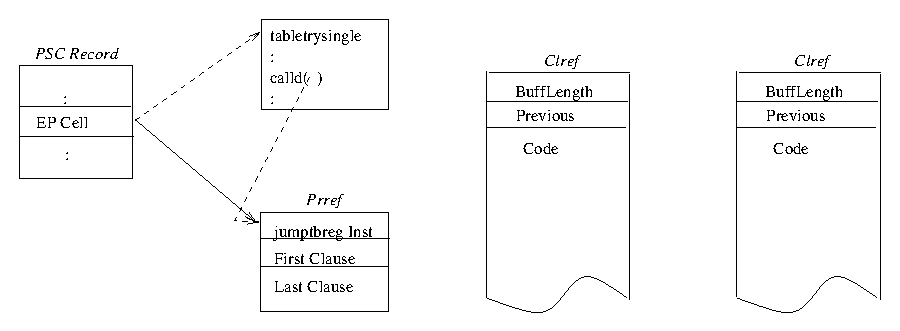
\epsfig{file=figures/dynamic-code.eps}
\caption{Schematic Picture of XSB's Dynamic Code Layout}
\label{fig:dynamic-code}
\end{figure}

(Rewritten 7/05 by DSW)

A dynamic predicate $p$ is stored differently from a compiled
predicate.  A dynamic predicate is stored as WAM bytecode with a
possibly complex index structure.  The entry point field of a psc
record for a (non-tabled) dynamic predicate points to a {\em Predicate
Reference} structure (PrRef), whose first field contains a bytecode
instruction that enters the executable code defining the dynamic
predicate.  (The instruction is a fail if there are no clauses at
all.)  If the code is a trie (when using trie indexing), this
instruction is a jump to the root trie-node.  If the code is regular
dynamic code, the instruction is a jumptbreg, which saves a pointer
(actually displacement) to the current choice-point in a register (made
to be the next unused argument register) for use by cuts, and then
jumps to enter the code that implements the asserted clauses.

If the dynamic predicate is tabled, then the psc entry point points to
a ``table wrapper'' structure which contains code that simulates a
single tabled clause that ``calls'' the PrRef.  Effectively, the
assert code simulates a transformation:
\begin{center}
:- table p/n.
\[
p(\vec{X}):- p_{dyn}(\vec{X}). 
\]
\end{center}
where $p_{dyn}(\vec{X})$ is the dynamic code asserted to $p(\vec{X})$.

The second and third fields of the PrRef contain pointers to
(respectively) the first and last clauses in the chain of all clauses
in the dynamic predicate, which allow fast access to the last clause
of the predicate for the assertz operation.

Figure \ref{fig:dynamic-code} shows a simple layout.

Assert (a/z) works by first using the function
assert\_code\_to\_buff\_p to generate code into a buffer, and then using
the function assert\_buff\_to\_clref\_p to link the buffer into the index
structure for the clauses already there.

The function assert\_code\_to\_buff\_p is a simple compiler of Prolog
clauses into WAM bytecode written in C.  It treats every clause as
though it had a single literal for its body.  This means that facts
are compiled close to optimally, and clauses with a single literal are
also compiled very much as the general compiler would compile them,
except that the assert\_code\_to\_buff\_p compiler uses a simpler
register allocation strategy.  If a clause has a complex body, then
the body will be compiled as a single call to the ``,'' (or
conjunction, or or, or if-then-else, or whatever control) predicate.
Cuts are supported by transforming the clause to have an extra
argument which is the choice-point address (actually displacement) to
use when cutting (with put(tp)breg).  This address is set during
execution by the jumptbreg that initially enters the dynamic code.

The more complex operation of adding the code into the indexing
structure for the dynamic predicate is done by the function
assert\_buff\_to\_clref\_p.

We'll first dispose of the rather simple case in which there is no
index on the dynamic predicate (obtainable only by explicitly
declaring an index of 0.)  In this case, a {\em Clause Reference Type
0} (ClRef0) record is created.  Its format is as follows:
\begin{verbatim}
        ClRef0 (for unindexed asserted code):
                -8: length of buffer (+0)
                -4: Addr of previous ClRef (or PrRef)
                0: Trymeelse-type instruction, for chain
                4: (cont) Addr of next ClRef on chain
                8+: BC for asserted clause
\end{verbatim}
In effect words are prepended to the buffer that contains the bytecode
for the asserted clause.  These words allow the buffers to be kept in
a doubly linked chain.  The first word is the length of the entire
buffer, including the bytecode; the second is the address of the
ClRef0 for the previous clause on the chain (or the PrRef if it is the
first clause); the third and fourth make up a bytecode instruction,
which will be a noop if it is the only clause, a trymeelse if it is
the first of several clauses, a retrymeelse if it is a middle of
several clauses, and dyntrustmeelsefail if it is the last of several
clauses.  The second words of each of these instructions naturally
form the forward chain.  (The noop has an argument that tells it to
skip the next word; the dyntrustmeelsefail has a second argument that
it ignores.)  Now branching to the first ClRef0 will result in the WAM
backtracking through the clauses in the predicate.  Also, it is now
easy to update this structure: asserta adds a buffer to the beginning
of the chain, modifying the instructions accordingly.  Assertz does
the same for the end of the chain.  Retract (brutal) can remove a
clause anywhere in the chain, since it is doubly linked.

Next we turn to considering how indexed clauses are represented.  In
XSB a predicate may have multiple indexes.  In this case if a given
call has arguments bound enough for the first index to apply, it will
be used; if not, it will see if the second index can be used and, if
so, will use it, etc.  This means that a single clause may have
multiple indexes and so may be on multiple different hash chains.
(The indexes we are describing here are all hash indexes.  Trie
indexing is available, but that uses a completely different data
structure described (I hope) elsewhere in this document.)

So each clause in an indexed predicate has a buffer called the {\em
Clause Reference Index} structure (ClRefI).  It contains its bytecode,
which is prefixed by links for the hashing chains for each index.  The
format is as follows (where NI is the Number of Indexes):
\begin{verbatim}
        ClRefI (for an indexed clause):
                -8: length of buffer (+3)
                -4: Addr of previous ClRefI on all chain
                0: Try-type instruction, for all subchain
                4: (cont) Addr of next ClRefI on all subchain
            For each index we have the following four fields: 
                8: BC noop(14) to skip next NI*8-2 bytes
                12: Addr of previous ClRefI on bucket chain
                16: Try-type instruction, for hash bucket subchain
                20: (cont) Addr of next ClRefI in bucket,
                    or back to SOB rec if last
                24: BC noop(6) to skip next (NI-1)*8-2 bytes
                28: Addr of previous ClRefI on bucket chain
                32: Try-type instruction, for hash bucket subchain
                36: (cont) Addr of next ClRefI in bucket
           NI*16+8: BC for asserted code
\end{verbatim}

So a clause with NI indexes is prefixed by 4+4*NI words.  Again the
first word is the length of the buffer (or'ed with 3 to indicate that
it is a ClRefI buffer); the second word is a pointer to the ClRefI of
the previous clause in this predicate; the third and fourth words are
a trymeelse-type bytecode instruction (again a noop, try, retry, or
trust, depending on its location in the chain) whose second word
participates in the forward chain of all clauses in the predicate.
Again branching to the address of the first ClRefI structure (note
that is a try-retry-trust chain) will backtrack through all the
clauses.  However, since a trymeelse-type instruction falls through to
execute the bytecode of the clause to try, when it does, we have to
jump to the actual byte code.  So the 5th word is a jump (here called
a noop with a parameter to say how many words to skip forward) to
cause the WAM to jump over the intermediate indexing chains.  Then the
6th word is the backwards link for the hashchain of this clause for
the first index; the 7th and 8th make up the trymeelse-type
instruction for the hashchain of the first index, and if there is
another index, the 9th word is a bytecode instruction to branch
forward the necessary number of words to skip those indexing
instructions to get to the WAM code for the clause.  And this
continues for as many indexes as there are.

So the question now is how the hashing is done, and the hashchains are
accessed and maintained.  This is done with {\em Clause Reference Type
1} (ClRef1) records (also know as SOB records, for SwitchOnBound, the
name of the WAM indexing instruction in XSB.)  The format is as
follows:
\begin{verbatim}
        ClRef1 (for group of indexed clauses, aka SOB record):
               -8: length of buffer (+1)
               -4: Addr of previous ClRef (or PrRef)
                0: Try-type instruction, for chain
                4: (cont) Addr of next ClRef on chain,
                        if trust-type then ptr to prref, if first-level
                        SOB, or ptr to previous enclosing SOB+20  
                8: BC switch-on-bound instruction (drop thru if var)
                11: (cont) arg(s) to index on
                12: (cont) address of Hash Table
                16: (cont) size of Hash Table
                20: BC jump to...        (or fail if empty)
                24: (cont) Addr of first ClRefI on all subchain
                    or to ClRef1 for next index
                28: Addr of last ClRefI on all subchain
                32: Number of clauses accessible thru this hash table
                36+: Hash Table
\end{verbatim}

In an indexed predicate ClRef1 blocks take the place of ClRef0 blocks
for unindexed predicates.  In the simplest case (of one (small) index
with all the clauses ground on the indexed argument) there will be
only one such block.  Again the first word is the length and type; the
second is the backward link in the ``all'' chain (when it becomes
necessary), and the third and fourth are the trymeelse-type
instruction for the all chain.  (In the simple case we are now
discussing, this would be a noop, since there would be only one block
on this chain.)  The interesting part is the WAM SwitchOnBound
instruction in words 5-8.  This instruction checks its argument (the
one it's indexing on, in a register) to see if it's ground (or
sufficiently instantiated to be used.)  If so, it hashes the functor
symbol (or whatever), finds the corresponding entry in the hash table
(13th and following words in this block), and branches to that
address.  That address will point to a chain of ClRefI blocks for the
clauses in that hash bucket.  If the argument is not bound, and so
cannot be indexed on, it falls through, to the 5th word in the block.
The 5th and 6th words contain a bytecode instruction which will branch
to the appropriate code to try next (or fail if there are no clauses
in this hashtable at all.)  If this is the last index to try, then it
will be a branch to the ClRefI block of the first asserted clause
(i.e., the try-chain containing all the clauses.)  If there is another
index to try, it will branch to another chain of ClRef1 (i.e., SOB)
records.  And the process continues.

We may need multiple ClRef1 (i.e., SOB) blocks chained through the
try-type instructions of their 3rd words.  Consider a sequence of
clauses: p(a),p(b),p(X),p(c),p(d), indexed on the (only) argument.
These will be represented with first a ClRef1 (SOB) block for p(a) and
p(b), then a ClRef0 block for p(X), and then another ClRef1 (SOB)
block for p(c) and p(d).  So one can think of this as being compiled
to be something like:
\begin{verbatim}
p(X) :- p1(X).           p1(a).
p(X).                    p1(b).
p(X) :- p2(X).
                         p2(c).
                         p2(d).
\end{verbatim}
where p1/1 and p2/1 are ``fully'' indexed.  Note that something like
this is required to preserve the order of clauses as demanded by Prolog
semantics.

At any point we can add a new ClRef0 or ClRef1 block to the chain of
these blocks.  For example consider assertz, adding a new ClRef1 (SOB)
at the end of the chain would ``close off'' the previous ones (since
assertz won't add to them any more,) and will start a new index for the
subsequently assertz-ed clauses.  This is useful for handling
predicates that get very many clauses asserted to them.  The idea is
that when a hashtable fills up, we will create another hashtable
that's twice as big as the previous one and just add it as the next
ClRef1 (SOB) block.  So in the 12th word (displacement 32) of an SOB
block is maintained the number of clauses in that hashtable, and when
it gets to be too many, a new larger SOB is allocated and added to the
end (for assertz, or the beginning for asserta.)  In this way, we get
a poor man's version of extensible hashing very easily.

Assert and retract manipulate this data structure to maintain its
consistency and correctness.  Both assert and retract operate directly
on these data structures when they are called.  Note that this means
that there may be references to these data structures in the
choice-point stack when the structures are modified.  In such cases
there may be problems.  For assert, structures are only extended.  We
have been careful to try to be sure that assert will always leave the
data structures in a state that is consistent for any computation
waiting on the choice-point stack.  So the semantics of asserting into
a clause when backtracking through it is not specified (and surely
weird), but at least the user should get something.  For retract, the
situation is more serious.  Since retract removes buffers and there
may be pointers to them from the choice-point stack, the system will
crash in some of these cases.  There is a version of retract, called
retract\_nr (for ``No Reclaim'', I believe), that leaves all buffers in
place, overwriting code with fail instructions to get the effect of
removing clauses but not changing the data structure.

\subsubsection{Multi-threading and Dynamic Code}
In the multi-threading engine, dynamic code may be shared (or global)
or private (or local.)  Shared dynamic code means that every thread
will see, and operate, on the clauses of the predicate.  Private
dynamic code means that each thread will work with its own version of
the predicate, not seeing any clauses in any other thread's version.
Dynamic code is private by default.  The user may declare a predicate
to be shared with a declaration:
\begin{verbatim}
:- thread_shared Name/Arity.
\end{verbatim}
Note that the {\em predicate} is shared or private, so all threads
must agree on the shared/private status of the predicate.

For shared dynamic code, we have tried to make assert (-a and -z)
thread-safe.  (Retract is {\bf not} thread-safe and must be used with
great care.  See previous discussion.)

For private dynamic code, both assert[a/z] and retract[all] are
thread-safe.  Private code is implemented by interposing a ``dispatch
table'' between the jump from the psc record and the PrRef (or
tabletrysingle code).  There is an instruction switchonthread that
branches through thte table based on the current thread.  See the
section below on private tables and dynamic code for details.

For shared predicates assert (and retract) use a mutex to lock out
other code modifiers when they are manipulating the dynamic data
structure.  However, readers are not locked out, so there is a
possibility of a reader of a dynamic predicate being interrupted {\em
at any point} by assert, which then changes the data structure the
reader is looking at.  We separate the issues for assertz and asserta.
For assertz, we don't need locks.  We need only have a single word
assignment be atomic.  We can set up the data structures so that
everything currently there is unchanged, except the dyntrustmeelsefail
instruction that must be changed to a retrymeelse instruction.  We can
change the second word of the dyntrustmeelsefail without bothering a
reader since that word is ignored in its execution.  Then by changing
the first word of that instruction atomically, the data structure will
be correct before and after that single assignment.  So by doing
things in this order, we can ensure that the assertz does not
interfere with any reader.  The other possible situation, that with
one clause (a noop) being changed to trymeelse, can be handled
similarly.

The more difficult issue is with asserta.  Here (in the general case)
we have an existing trymeelse instruction and we need to add a new
trymeelse for the new clause being added and change that old trymeelse
to a retrymeelse.  Here there is a problem in that we have two words
in the old data structure that need to be changed, and both are used
by the executing code.  We need to change the pointer to the old first
clause to point to the new first clause, and we need to change the
instruction of the old first clause to become a retrymeelse.  No
matter in which order we do them, the data structure between the
assignments will be inconsistent for a reader.  (Note a similar
situation can occur when the second clause is added, and a noop is
changed to a dyntrustmeelsefail.)

To solve this problem, we require that readers acquire the lock used
by assert (and retract.)  So a reader needs to acquire the lock before
it branches to a trymeelse instruction (or noop instruction) that
might be changed, must keep it till it has completed execution of the
trymeelse (or noop) instruction, and it must then release the lock.
This will guarantee that the reader sees a consistent data structure.

So in the multi-threaded engine, the following changes have been made
to implement this strategy.  The jumptpreg instruction used to enter
dynamic code gets the lock.  New instructions have been created:
dyntrymeelse, dynnoop, and dynfail.  These instructions are used
instead of their correspondents for the instructions that cause the
execution of clause bytecode in ClRefI buffers.  They do their work
and then as the last thing, release the lock (if it is held.)  Dynfail
is necessary for releasing the lock when indexing determines that no
code is executed, so the hashtables are initialized to point to a
dynfail instruction to ensure the lock is released in this case.

These instructions may be called in cases in which the lock has
already been released, so they keep track of whether they have the
lock (with i\_have\_dyn\_lock) and release it only if they do.  With a
sequence like asserta(p(b2)), asserta(p(b1)), asserta(p(X)),
asserta(p(a2)), asserta(p(a1)), which generates multiple ClRef1 (and
0) blocks, there will be multiple dyntrymeelse instructions executed
when backtracking through it.

\subsubsection{Multi-threading and Private Tables and Dynamic Code}

In the multi-threading engine, predicates default to being
thread\_private.  This means that each thread has its own version of 


\subsection{Storage of Compiled Code in Program Segments}
%===========================

A program segment normally corresponds to a text/index segment in the 
byte code file.
The format of a program segment is shown in Figure \ref{f:programseg}.
All program segments in memory are chained together. The C variable
{\tt inst\_begin} points to the head of the chain, and 
{\tt last\_text} points to the tail of the chain. Newly loaded
segments are at the end of the chain.

\begin{figure}
\begin{verbatim}
              ----------------      ------------        -----------
          /   | next seg     |  +-->|        --|------->|       --|---+
          |   ----------------  |   ------------        -----------   |
          |   | previous     |  |   |size (+8) |        |size (+8)|   |
  16     {    ----------------  |   ------------        -----------   |
  bytes   |   | index blocks |--+   |          |        | try     |   |
          |   ----------------      | hash     |        | retry   |   |
          \   | size (+16)   |      | table    |        | trust   |   |
  codeptr --->----------------      |          |        -----------   |
          /   |              |      ------------                      |
          |   |              |                          -----------   |
          |   | instructions |                          | 0 (end) |<--+
          |   |              |                          -----------
  text_  {    |              |                          |size (+8)|
  bytes   |   |              |                          -----------
          |   |              |                          |  hash   |
          |   |              |                          |  table  |
          |   |              |                          |         |
          \   |              |                          -----------
              ----------------
\end{verbatim}
\caption{Format of a Program Segment in Memory}
\label{f:programseg}
\end{figure}

Each index block contains a hash table and possible added instructions
({\tt try, retry} and {\tt trust}). The size of the hash table
($T$, number of buckets) is computed from the number of clauses ($N$) by the C
function {\tt hsize} with the following steps:

\begin{itemize}
  \item If $N>64$, $N' = N/2$;
  \item If $16 < N \leq 64$, $N' = N$;
  \item If $N \leq 16$, $N' = 2N+1$;
\end{itemize}

$T$ is then the first prime number greater than or equal to $N'$.


\subsection{Forms of Predicate Definitions}
%==========================================

\begin{enumerate}
    \item compiled predicates --- see Figure \ref{f:cmppred}

\begin{figure}
\begin{verbatim}
        One clause:
             -------------------------------------------
             | compiled clause: instructions ... ...
             -------------------------------------------
   
        N clauses, N > 1:
             -------------
             | try       |
             -------------
             | retry     |    \
             -------------    |
                 ...          |   N - 2 retry
             -------------    |
             | retry     |    /
             -------------
             | trust     |
             -------------

             -------------------------------------------
             | compiled clause: instructions ... ...
             -------------------------------------------
             .............

             -------------------------------------------
             | compiled clause: instructions ... ...
             -------------------------------------------
\end{verbatim}
\caption{Format of a compiled predicate}
\label{f:cmppred}
\end{figure}

    \item compiled clauses have the following forms (may have more):
\begin{verbatim}
       a.   allocate             b.
            ......                   ......
            other instr              other instr
            ......                   ......
            deallocate               execute or proceed
            execute or proceed
\end{verbatim}

   * the number of clauses may not be the same as in the source,
     because of the source transformations for cut and index.

    \item Clause reference in buffer: (generated by "db.p")
\label{pg:clauseref}
        without indexing:

\begin{verbatim}
         .....................
     -4  : buffer size       :
         -------------------------------------------
      0  | noop/trymeelse's  |  (next clause ref)  |
         ------------------------------------------------
      8  |pil instructions   ... ...
         ------------------------------------------------
\end{verbatim}

	The first two words are reserved for a choice instruction
	({\it trymeelse, retrymeelse, trustmeelsefail}) or an {\it noop 2}
	instruction when there is only one clause in the chain.

        With indexing, there are two chains: one for all clauses
	of the predicate and the other for clauses in the same has bucket.

\begin{verbatim}
         .....................
     -4  : buffer size       :
         ------------------------------------------
      0  | noop/trymeelse's  |  ( "all" chain )   |
         ------------------------------------------
      8  | noop/trymeelse's  |  ( bucket chain)   |
         ----------------------------------------------
     16  |pil instructions   ... ...
         ----------------------------------------------
\end{verbatim}

	When a static predicate is converted to dynamic, the compiled
	code is made a single clause reference (with newly allocated
	16 bytes clause reference buffer).
\end{enumerate}


\subsection{The Stack Spaces}
%============================

Stack spaces are used for global stacks, local stacks, choice point
stacks and trail stacks.  Each stack space is associated with one
thread. In the case of sequential mode, there is only one thread and
hence there is only one stack space.  A stack space is therefore
identified by the thread control block (page \pageref{pg:tcb}) of the
associating thread.  Each stack space is divided into two halves: one
for global and local stacks and the other for choice point and trail
stacks.  The two halves of a stack space are not necessarily adjacent
to each other.  Figure \ref{f:stackspace}(a) shows the format of a
stack space.  The boundaries of the two halves of the stack space (the
bottoms of the four stacks) are stored in the thread control block, as
shown in the figure ({\tt T.memory, T.lstack, T.trail}, and {\tt
T.memend}).

A stack space is normally allocated as a contiguous memory space
block.  Because a thread will be suspended when it creates a branch
point until all its children terminate, the unused portion of the
space of the parent thread can be used as the stack space of one child
(Figure \ref{f:stackspace}(b) ). We say in this case the child
{\tt shares} the stack space with its parent, although it really
allocates the stacks within the parent stack space.  Due to this
optimization technique, the two halves of a stack space may not be
adjacent to each other but some gaps are left in between.


{\tt hreg} always points to the first free space on the global stack,
and is initially set to {\tt T.memory}.  {\tt hbreg} is also set to
{\tt T.memory} initially.  {\tt ereg} always points to the bottom of
current environment, and is initially set to {\tt T.lstack}-1.
However, {\tt ebreg} is set to be the same as {\tt T.lstack}
initially, since it always points to the top of the environment before
the last choice point.  {\tt trreg} points to the first free space and
is initially set to {\tt T.trail}.

The choice point stack is initialized to contain a root choice point,
only three fields of which are significant: {\tt pcreg} field pointing
to a {\tt halt} (in first stack space), {\tt hreg} field containing
initial {\tt hbreg} value, and {\tt ebreg} field containing the
initial {\tt ebreg} value.  The last two fields are used for cut.
{\tt breg} points to the bottom of the last choice point record, and
points to the root choice point initially.


\begin{figure}
\begin{verbatim}
           +-------------+<-- T.memend               +------------+
    Choice |      :      |                           |T1 CP stack |
    Point  |      :      |                           + - - - - - -+
    Stack  |      :      |                           |T2 CP stack |
           |      V      |<- breg                    |            |
           |             | (top of stack)            |            |
           |             |                           |            |
           |             |                           |            |
           |      ^      |<- trreg                   |            |
           |      :      | (1st free word)           |            |
    Trail  |      :      |                           |            |
    Stack  |      :      |                           | T2 trail   |
           |-------------|<-- T.trail                + - - - - - -+
                                                     | T1 trail   |
    possible gaps here when the space                +============+
    is shared with the parent thread                 | T1 l. stack|
                                                     |            |
           |-------------|<-- T.lstack               + - - - - - -+
           |      :      |                           | T2 l. stack|
    Local  |      :      |<- ebreg                   |            |
    Stack  |      :      |<- ereg                    |            |
           |      V      |                           |            |
           |             |                           |            |
           |             |                           |            |
           |      ^      |<- hreg                    | T2 g. stack|
           |      :      |  (1st free word)          + - - - - - -+
    Global |      :      |<- hbreg                   |            |
    Stack  |      :      |                           | T1 g. stack|
           +-------------+<-- T.memory               +------------+

                (a)                                       (b)
\end{verbatim}
\caption{The Stack Space Format}
\label{f:stackspace}
\end{figure}


\subsection{Emulator Flags}
%==========================

These flags are implemented in C but are accessible through {\it stat\_flag}
and {\it stat\_set\_flag} predicates. They are listed in the Appendix
\ref{s:emuflags}.


\subsection{Format of Buffers}
%=============================


A buffer is simply a block of memory space within the permanent
space ({\it permanent buffer}) or in the global stack of a thread
({\it temporary buffer}). A buffer is identified by a number
whose value is the initial address of the buffer.
When a buffer is allocated,
the first word of the buffer stores the size of the buffer. 
It can be overwritten if you wish.


\section{System Libraries} \label{sec:libs}
%==========================================

\subsection{Interpreter Flags}

The flags in Table \ref{t:interpflag} are implemented in the
interpreter, at the Prolog level. The first three flags have their
correspond emulator flags. They are repeated in the Prolog level in order
to store their symbolic names. It is important, therefore, to set
both interpreter flag and emulator flag in the same time, so that
consistency is preserved.

\begin{table}\centering
\begin{tabular}{l|l}
\hline
Name                &  Function \\
\hline
current\_input  & ep points to the psc record of the current input file name\\
current\_output & ep points to the psc record of the current output file name\\
current\_module & ep points to the psc of the current module name entry; \\
\hline
\end{tabular}
\caption{Interpreter Internal Flags}
\label{t:interpflag}
\end{table}

\subsection{Format of Recorded Terms}
%====================================

The format of recorded terms under a record key is given in Figure
\ref{f:record}.
A database reference for a recorded term
is a pointer to the node for that term.

\begin{figure}
\begin{verbatim}
       -----------------------------------------
       |T_RKEY|      ...         | ep:       --|---+
       -----------------------------------------   |
        Psc for the record key                     |
                      +----------------------------+
                      |
            +---------V--+<---+
Header      | next     --|--+ |
node        +------------+  | |         When empty, the next/prev
       +----|-previous   |  | |         fields of the header node
       | +->+------------+  | |         point to itself.
       | |  | buffer=0   |  | |
       | |  +------------+  | |
       | |  | size       |  | |
       | |  +------------+  | |
       | |                  | |
       | |  +------------+<-+ |
       | |  | next     --|--+ |
       | |  +------------+  | |
       | +--|-previous   |  | |
       | +->+------------+  | |   +------------------------------------+
       | |  | buffer   --|--)-)-->| a copied term                      |
       | |  +------------+  | |   +------------------------------------+
       | |  | size       |  | |
       | :  +------------+  : |
       | :  ...   ...       : |
       | :  ...   ...       : |
       | :  ...   ...       | |
       | |  +------------+<-+ |
       | |  | next     --|----+
       | |  +------------+  
       | +--|-previous   |
       +--->+------------+        +------------------------------------+
            | buffer   --|------->| a copied term                      |
            +------------+        +------------------------------------+
            | size       |
            +------------+  
\end{verbatim}
\caption{Format of recorded terms}
\label{f:record}
\end{figure}


\section{Modifying the System} \label{sec:modification}
%======================================================

\subsection{Adding a Hard Built-in Predicate}
%==========================================

\begin{enumerate}
  \item At the beginning of {\tt emu/builtin.c}, add

	\demo{       \#define {\it Name} {\it number}		}

  \item Add in one case entry in {\tt emu/builtin.c} to implement the
	 built-in.
  \item In {\tt syslib/machine.P}, add a Prolog interface to it.
  \item In {\tt cmplib/builtin.P}, add an inline entry for it.
  \item Modifying the documentation appropriately.
\end{enumerate}

The style of built-in predicates: they are normally in a much lower level
than standard predicates as those provided at the language level. All
built-in predicates are deterministic, never fails, and usually do not perform
tag checking or mode checking. When C procedure that implements built-in
predicates returns a 0 value, the emulator will fail the current path
and backtrack; otherwise the emulator assumes the built-in predicates
succeed and continue the current instruction flow.

\subsection{Adding a New Abstract Machine Instruction}
%-----------------------------------------------------

\begin{enumerate}
  \item In {\tt emu/inst.h}, add a line

	\demo{     \#define {\it name} {\it opcode}		}

  \item In {\tt emu/inst.c}, add a line

	\demo{     set\_inst({\it name}, {\it argtype});	}

  \item In {\tt emu/emulator.i}, add a case that
          implement the new instruction.
  \item In {\tt cmplib/asm\_inst.P}, add one clause
          in the predicate {\tt asm\_inst/4}.
  \item Modify the compiler to generate such an instruction.
  \item Modifying the documentation appropriately.
\end{enumerate}

\subsection{System Debugging}
%============================

There are three emulator command line options for system debugging purpose.
These options are available only if the system is compiled with the flag
``-DDEBUG''.  They are listed below:

\begin{description}
  \item[-t] Turn on WAM instruction tracing: print every WAM instruction
	on the standard output before executing it.
  \item[-T] Turn on system debugger and call tracing. The system will stop
	at each entry of a call to a predicate and wait for user interaction.
	A list of interactive command can be printed by typing ``h''.
  \item[-d] Disassemble the input byte code file and exit immediately.
  \item[-S] Turn on printing information when creating, awaking, and deleting
	a thread.
\end{description} 



\section{Tabling Extensions} \label{sec:tabling}
%===============================================

Descriptions of extensions for tabling will be added (lazily!), as I
write them up for other purposes.

\subsection{Table Management Routines}

Figure~\ref{stack-layout.ps} shows the high-level structure of xsb memory.

\begin{figure}[htbp]
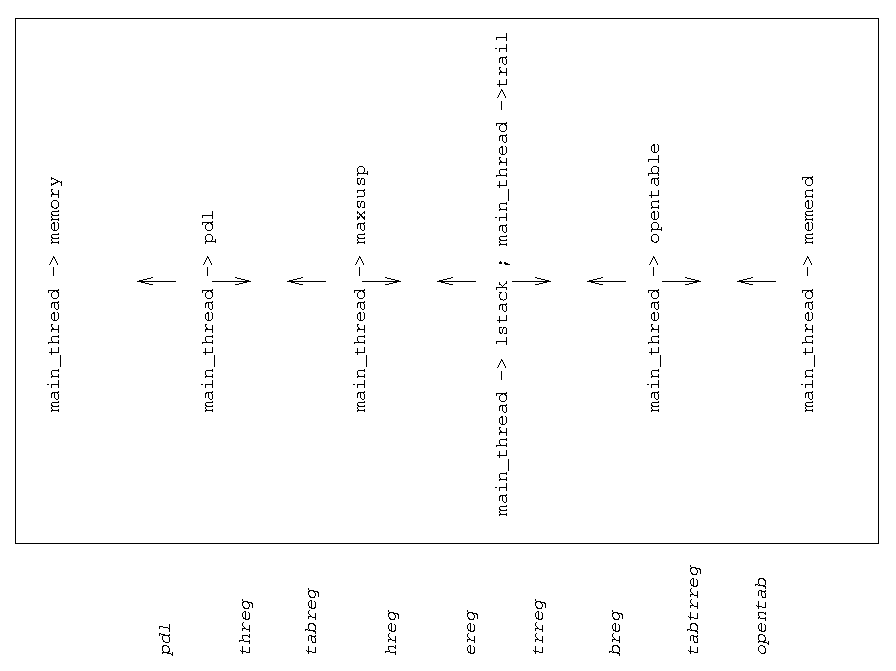
\epsfig{file=figures/stack-layout.eps}
\caption{Schematic Picture of XSB memory layout}\label{stack-layout.ps}
\end{figure}

Figure~\ref{tabspc.ps} shows the high-level structure of the table
space.  

\begin{figure}[htbp]
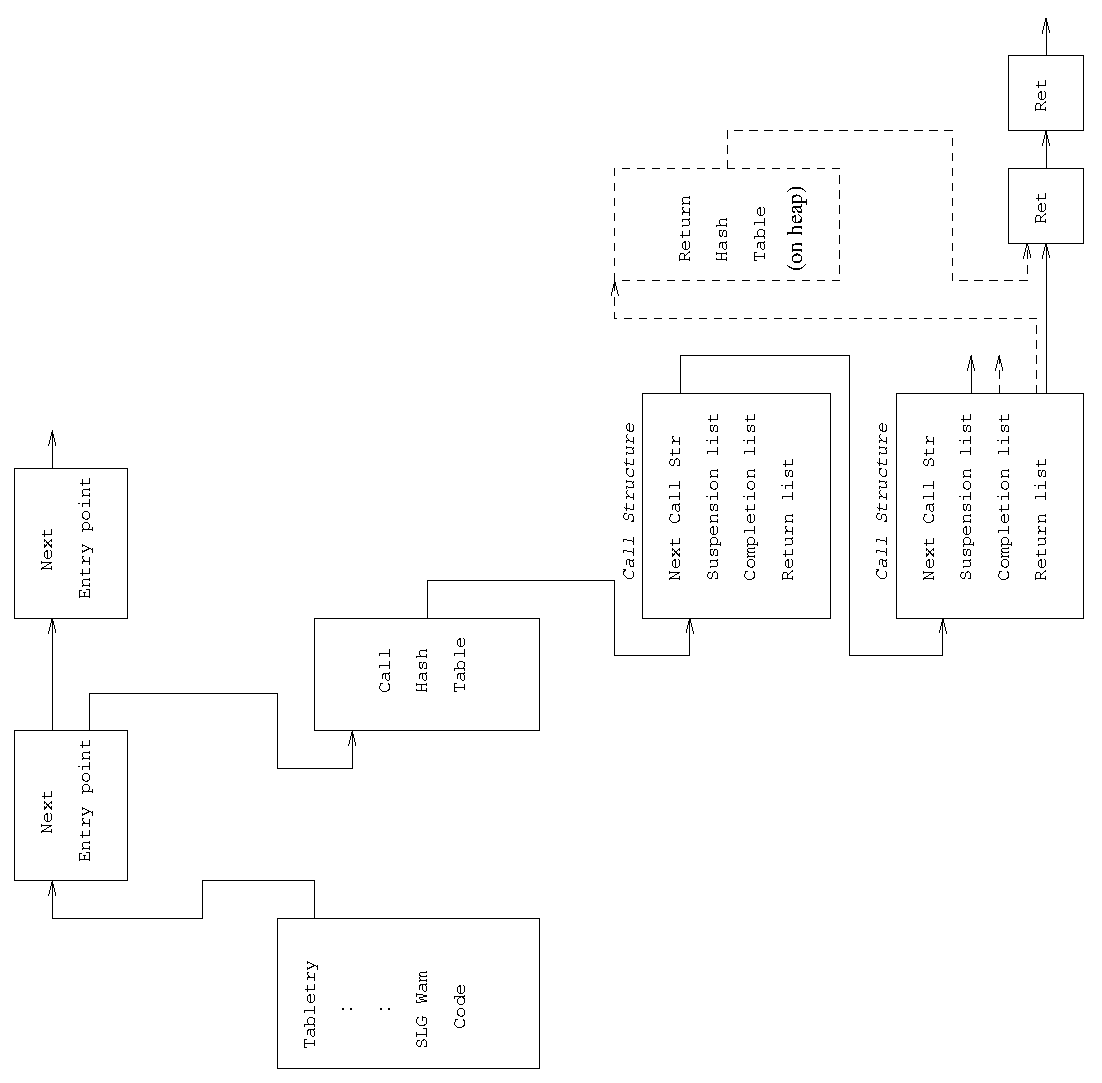
\epsfig{file=figures/tabspc.eps}
\caption{Schematic Picture of Table Space}\label{tabspc.ps}
\end{figure}

\begin{verbatim}
Table management Routines
	
	check_table_stack_overflow in choice.h
	saveinfo in xinst_fun copies from global.local into tablespace
	load_solution in xinst_fun copies into global.local from tablespace
	In addition to using table registers, they use the fact that
tables lie in virtual memory BELOW WAM stacks.  They will need to be
changed to make a check that tables are above WAM stacks.
	

Table Information Structures and pointers to them (tip)
	(grep on tip)

	-- typedef in xmacro.h, along with access macros.

	-- emu/psc.c contains a routine for finding a tip from a psc
pointer (pscs are explained in PSB tech ref manual).

	-- load_seg.c contains routines for initializing these
structures, using info from .O files.

	-- emu/builtin.c contains several built-ins which access
information in tables through table information structures, and
'tip's, which are pointers to them.  The built-ins are used mostly in
lib/tables.P.  (built-ins generally are described in the PSB tech
reference manual).

Memory Management (such as it is) is in memory.h
	Space for program code is malloced as needed.
	Stack space is allocated once in init.c

Table abolishing routines.
	In tables.P

Debugging Routines
	In debug.c

hashindex.h
	This file culls out all call and return indexing routines, and
routines to traverse return lists.

\end{verbatim}

\subsection{Instruction-level Debugging}
%==========================-============

The instruction level debugger is a powerful aid to improving the
emulator.  If you add or modify existing SLG-WAM instructions, you
will sooner or later need to use it or something like it.

Instruction level debugging can be invoked from the interpreter in
two ways.  The most general way is to use the predicate {\tt
set\_pil\_on/0} from tables.P.  The goal
\begin{center} 
{\tt set\_pil\_on,p(X) }
\end{center}
will begin an instruction level trace with the call of {\tt p/1}.
Alternately adding the preprocessor directive
\begin{center}
\#define XTRACE
\end{center}
will begin an instruction level trace as soon as {\em xwammode} is
entered.  This condition holds from the time the first table in an
evaluation is entered until the time the last table is completed.

The debugger itself allows one to examine stacks and registers at each
instruction, to skip ahead a specified number of instructions, or to
set a memory or register watch to a particular value.  It is suggested
that debugging be done from a shell that allows scrolling and
searching, such as a shell invoked from emacs.

Each instruction is printed out in the format
\begin{center}
{\em instruction-number instruction-address  instruction  parameters}
\end{center}
The instruction printed out will be executed {em next}.  After an
instruction or instructions are printed out, the debugger waits for a
prompt from the user.  Some useful values are presented below, but see
debug.c for a full set.  All addresses are assumed to be in
hexadecimal.

\begin{itemize}
	\item {\em q} quits 	
\item {\em d} disassembles all loaded
code.  	
\item {\em r num} prints the cell value, and deref'ed value of
a register.  	
\item {\em R num} prints the cell value, and deref'ed
value of a register.  	
\item {\em v num} prints the value of a
permanent variable.  	
\item {\em a d num} prints the value at an
address.  	
\item {\em 1} prints table stack starting from tabreg.
Several lines are printed out and the user is prompted to continue.
\item {\em 2} prints table heap starting from threg.  Several lines
are printed out and the user is prompted to continue.  
\item {\em P}
prints unification stack starting from pdlreg.  Several lines are
printed out and the user is prompted to continue.  	
\item {\em P}
prints unification stack starting from pdlreg.  Several lines are
printed out and the user is prompted to continue.  	
\item {\em p}
prints global stack starting from hreg.  Several lines are printed out
and the user is prompted to continue.  	
\item {\em e} prints local
stack starting from top of stack.  Several lines are printed out and
the user is prompted to continue.  	
\item {\em t} prints trail
starting from trreg.  Several lines are printed out and the user is
prompted to continue.  	
\item {\em c} prints choice point stack
starting from breg.  Several lines are printed out and the user is
prompted to continue.  
\item {\em C} prints choice point stack
starting from bfreg.  Several lines are printed out and the user is
prompted to continue.  	
\item {\em o} prints open table stack starting
from openreg.  Several lines are printed out and the user is prompted
to continue.  	
\item {\em S} prints values of registers.  	
\item {\em k num} skips {\em num} instructions, printing each instruction.
\item {\em K num} skips {\em num} instructions, without printing each
instruction. 
\item {\em w regnum num} sets register watch
\item {\em W stacknum num} sets memory watch
\end{itemize}

The register watch and memory watch bear further explanation.  The
register watch prints out a message whenever the register has a
particular value.  This is useful for determining when a program
might backtrack to a certain environment, say, or when a particular
binding is trailed.  The memory watch is similar, but prints out a
message whenever a particular address changes value, and is useful for
catching when bindings occurs.

There are also hooks from the instruction level debugger to the
interpreter level debugger, although these hooks can be shaky when
tabled code is traced, or when the dynamic loader is used.  See
debug.c for details.

When tracing tabling instructions, sets of printfs are spewn out when
the directives
\begin{center}
\#define XPIL
\#define XPIL1
\end{center}
or
\begin{center}
\#define OLDTTRACE
\end{center}
are written in main.c  XPIL dumps information about table
instructions, XPIL1 dumps information about indexing and table copy
subinstructions, and OLDTTRACE prints out information about table
calls and solutions.

\section                 {Miscellaneous}
%                        ===============

\subsection{Save Status File Format}
%==================================

This subsection is to be rewritten due to the {\tt save} feature
is not tuned to the \version \mbox{} yet. The old format given below does
not work for the current version.

\begin{verbatim}
    4: 0x11121307        magic number

    4: pspace                start addr of pspace;
    4: maxspace                size of pspace;
    4: memory                start addr of local and heap stack
    4: maxmem                size of local and heap stack
    4: tstack                start addr of trail stack
    4: maxtrail                size of trail stack

    4: breg
    4: ereg
    4: hreg
    4: trreg
    4: hbreg
    4: cpreg
    4: pcreg

    4: nil_sym
    4: list_str
    4: list_psc
    4: comma_psc
    4: interrupt_psc
    8: trap_vector

    4: curr_fence        current top of pspace
    4: heap_used
    4: stack_used

    4: global_pair        ??? need to modify
    4: mod_list
    4: temp_list

    40: flags
    12: reg

subtotal: 160
pspace:   used portion
t-stack:  used portion
heap:     used portion
stack:    used portion
\end{verbatim}

\begin{thebibliography}{[8]}
 \bibitem[1]{sbprolog}
	Edited by Saumya Debray. {\it SB-Prolog Version 2.5 -- a user manual},
	September 1988.
\end{thebibliography}

\newpage

\appendix

\section		{Abstract Machine Instructions}
%			===============================

We list all abstract machine instructions below. All the instructions
are aligned with word (4 bytes) boundary with unused bytes padded.
This is necessary for running on machines with word alignment
restrictions such as Motorola 68000 (2 bytes alignment) or SPARC (4
bytes alignment). The size of instructions can be one, two or three
words. The opcode of the instruction takes the first byte in the first
(or the only) word, and the rest 3 bytes of the words are used for
arguments of one byte long. The second or the third word, if used,
always contain a single operand that requires the whole word.  

The
argument types listed in the table have the following meaning:

\begin{description}
  \item[A] one byte number for arity, size, built-in number, etc.
  \item[V] variable offset (one byte)
  \item[R] register number (one byte)
  \item[S] a structure (four bytes)
  \item[C] a constant (four bytes)
  \item[L] a label (address, four bytes)
  \item[G] a string
  \item[N] a number (integer, fast floating point, or ref to a boxed number. four bytes)
  \item[I] special; for the 2nd and 3rd arguments of switchonbound
  \item[P] pad, use a ``-'' in the table: the byte is not used (one byte)
  \item[PP] double pad, use two ``-'' in the table (two bytes)
  \item[PPP] triple pad, use three ``-'' in the table (three bytes)
\end{description}

\begin{tabbing}
Opcode\= Name Name Name \=Arg\=Arg\=Arg\= 2rd Word \= 3rd Word \= comments\kill
Opcode\> Name	\>A1 \>A2 \>A3 \>2rd Word\>3rd Word\>\hspace*{3em} Comments \\
\rule{\textwidth}{.01in}\\
0x00  \> getpvar	\> - \> V \> R \>   \>	 \>		\\
0x01  \> getpval	\> - \> V \> R \>   \>	 \>		\\
0x02  \> getstrv	\> - \> - \> V \> S \>   \>		\\
0x03  \> gettval	\> - \> R \> R \>   \>	 \>		\\
0x04  \> getcon		\> - \> - \> R \> C \>   \>		\\
0x05  \> getnil		\> - \> - \> R \>   \>   \>		\\
0x06  \> getstr		\> - \> - \> R \> S \>	 \>		\\
0x07  \> getlist	\> - \> - \> R \>   \>   \>		\\
0x08  \> unipvar	\> - \> - \> V \>   \>	 \>		\\
0x09  \> unipval	\> - \> - \> V \>   \>	 \>		\\
0x0a  \> unitvar	\> - \> - \> R \>   \>	 \>		\\
0x0b  \> unitval	\> - \> - \> R \>   \>	 \>		\\
0x0c  \> unicon		\> - \> - \> - \> C \>   \>		\\
0x0d  \> uninil		\> - \> - \> - \>   \>   \>		\\
0x0e  \> getnumcon	\> - \> - \> R \> N \>   \>		\\
0x0f  \> putnumcon	\> - \> - \> R \> N \>   \>		\\
0x10  \> putpvar	\> - \> V \> R \>   \>	 \>		\\
0x11  \> putpval	\> - \> V \> R \>   \>	 \>		\\
0x12  \> puttvar	\> - \> R \> R \>   \>	 \>		\\
0x13  \> putstrv	\> - \> - \> V \> S \>   \>		\\
0x14  \> putcon		\> - \> - \> R \> C \>   \>		\\
0x15  \> putnil		\> - \> - \> R \>   \>	 \>		\\
0x16  \> putstr		\> - \> - \> R \> S \>   \>		\\
0x17  \> putlist	\> - \> - \> R \>   \>	 \>		\\
0x18  \> bldpvar	\> - \> - \> V \>   \>   \>		\\
0x19  \> bldpval	\> - \> - \> V \>   \>   \>		\\
0x1a  \> bldtvar	\> - \> - \> R \>   \>	 \>		\\
0x1b  \> bldtval	\> - \> - \> R \>   \>	 \>		\\
0x1c  \> bldcon		\> - \> - \> - \> C \>   \>		\\
0x1d  \> bldnil		\> - \> - \> - \>   \>   \>		\\
0x1e  \> uninumcon	\> - \> - \> - \> N \>   \>		\\
0x1f  \> bldnumcon	\> - \> - \> - \> N \>   \>		\\
0x20  \>		\>   \>   \>   \>   \>	 \> not used	\\
---   \>		\>   \>   \>   \>   \>   \>		\\
0x47  \>		\>   \>   \>   \>   \>   \> not used	\\
0x48  \> getlist-tvar-tvar\>R\> R \> R \>   \>	 \>		\\
0x49  \> getcomma	\> - \> - \> R \>   \>   \> currently not used	\\
0x4a  \> getcomma-tvar-tvar\>R\>R \> R \>   \>   \> currently not used	\\
0x4b  \>		\>   \>   \>   \>   \>	 \> not used	\\
---   \>		\>   \>   \>   \>   \>   \>		\\
0x7f  \>		\>   \>   \>   \>   \>   \> not used	\\
0x80  \> getfloat	\> - \> - \> R \> N \>   \>		\\
0x81  \> putfloat	\> - \> - \> R \> N \>   \>		\\
0x82  \> unifloat	\> - \> - \> - \> N \>   \>		\\
0x83  \> bldfloat	\> - \> - \> - \> N \>   \>		\\
0x84  \>		\>   \>   \>   \>   \>	 \> not used	\\
---   \>		\>   \>   \>   \>   \>   \>		\\
0x99  \>		\>   \>   \>   \>   \>   \> not used	\\
0x9a  \> trys		\> - \> - \> A \> L \>   \>		\\
0x9b  \> retrys		\> - \> - \> A \> L \>   \>		\\
0x9c  \> trusts		\> - \> - \> A \> L \>   \>		\\
0x9d  \> neck		\> - \> - \> A \>   \>   \>		\\
0x9e  \> neck-putpbreg	\> - \> A \> V \>   \>	 \>		\\
0x9f  \> neck-puttbreg	\> - \> A \> R \>   \>	 \>		\\
0xa0  \> trymeelse	\> - \> - \> A \> L \>   \>		\\
0xa1  \> retrymeelse	\> - \> - \> A \> L \>   \>		\\
0xa2  \> trustmeelsefail\> - \> - \> A \>   \>   \>		\\
0xa3  \> try		\> - \> - \> A \> L \>   \>		\\
0xa4  \> retry		\> - \> - \> A \> L \>   \>		\\
0xa5  \> trust		\> - \> - \> A \> L \>   \>		\\
0xa6  \> getpbreg	\> - \> - \> V \>   \>   \>		\\
0xa7  \> gettbreg	\> - \> - \> R \>   \>	 \>		\\
0xa8  \> putpbreg	\> - \> - \> V \>   \>   \>		\\
0xa9  \> puttbreg	\> - \> - \> R \>   \>	 \>		\\
0xaa  \> jumptbreg	\> - \> - \> R \> L \>   \> used by dynamic preds\\
0xab  \> getarg-proceed \> - \> - \> A \>   \>   \> used by par-member	\\
0xac  \> getstring	\> - \> - \> R \> G \>   \>		\\
0xad  \> putstring	\> - \> - \> R \> G \>   \>		\\
0xae  \> unistring	\> - \> - \> - \> G \>   \>		\\
0xaf  \> bldstring	\> - \> - \> - \> G \>   \>		\\
0xb0  \> switchonterm	\> - \> - \> R \> L \> L \>		\\
0xb1  \> switchoncon	\> - \> - \> - \> L \>   \>		\\
0xb2  \> switchonstr	\> - \> - \> - \> L \>   \>		\\
0xb3  \> switchonbound	\> - \> - \> R \> I \> I \>		\\
0xb4  \>		\>   \>   \>   \>   \>	 \> not used	\\
0xb5  \>		\>   \>   \>   \>   \>   \> not used	\\
0xb6  \> suspend	\> - \> - \> - \>   \>   \> not used by compiler \\
0xb7  \> partry		\> - \> - \> A \> N \>   \>		\\
0xb8  \> terminate	\> - \> - \> - \>   \>   \> not used by compiler \\
0xb9  \>		\>   \>   \>   \>   \>	 \> not used	\\
---   \>		\>   \>   \>   \>   \>   \>		\\
0xd0  \>		\>   \>   \>   \>   \>   \> not used	\\
0xd1  \> movreg		\> - \> R \> R \>   \>	 \>		\\
0xd2  \> negate		\> - \> - \> R \>   \>	 \>		\\
0xd3  \> and		\> - \> R \> R \>   \>	 \>		\\
0xd4  \> or		\> - \> R \> R \>   \>	 \>		\\
0xd5  \> logshiftl	\> - \> R \> R \>   \>	 \>		\\
0xd6  \> logshiftr	\> - \> R \> R \>   \>	 \>		\\
0xd7  \> addreg		\> - \> R \> R \>   \>	 \>		\\
0xd9  \> subreg		\> - \> R \> R \>   \>	 \>		\\
0xd9  \> mulreg		\> - \> R \> R \>   \>	 \>		\\
0xda  \> divreg		\> - \> R \> R \>   \>	 \>		\\
0xdb  \> idivreg	\> - \> R \> R \>   \>	 \>		\\
0xdc  \>		\>   \>   \>   \>   \>	 \> not used	\\
---   \>		\>   \>   \>   \>   \>   \>		\\
0xdf  \>		\>   \>   \>   \>   \>   \> not used	\\
0xe0  \> putdval	\> - \> V \> R \>   \>	 \>		\\
0xe1  \> putuval	\> - \> V \> R \>   \>	 \>		\\
0xe2  \> getival	\> - \> - \> A \> S \>   \> not used by compiler \\
0xe3  \>		\>   \>   \>   \>   \>	 \> not used	\\
---   \>		\>   \>   \>   \>   \>   \>		\\
0xe6  \>		\>   \>   \>   \>   \>   \> not used	\\
0xe7  \> unexec		\> - \> - \> - \> S \> S \> not used by compiler \\
0xe8  \> call		\> - \> - \> A \> S \>   \>		\\
0xe9  \> allocate	\> - \> - \> - \>   \>   \>		\\
0xea  \> deallocate	\> - \> - \> - \>   \>   \>		\\
0xeb  \> proceed	\> - \> - \> - \>   \>   \>		\\
0xec  \> execute	\> - \> - \> - \> S \>   \>		\\
0xed  \> unexeci	\> - \> - \> - \> S \> S \> not used by compiler \\
0xee  \> executev	\> - \> - \> - \> S \>   \>		\\
0xef  \> calld		\> - \> - \> A \> L \>   \>		\\
0xf0  \> jump		\> - \> - \> - \> L \>   \>		\\
0xf1  \> jumpz		\> - \> - \> R \> L \>   \>		\\
0xf2  \> jumpnz		\> - \> - \> R \> L \>   \>		\\
0xf3  \> jumplt		\> - \> - \> R \> L \>   \>		\\
0xf4  \> jumple		\> - \> - \> R \> L \>   \>		\\
0xf5  \> jumpgt		\> - \> - \> R \> L \>   \>		\\
0xf6  \> jumpge		\> - \> - \> R \> L \>   \>		\\
0xf7  \> cases		\> A \> N \> N \>   \>   \> 
					10 bytes; not used in emulator \\
0xf8  \> fail		\> - \> - \> - \>   \>   \>		\\
0xf9  \> noop		\> - \> - \> A \>   \>   \>		\\
0xfa  \> halt		\> - \> - \> - \>   \>   \>		\\
0xfb  \> builtin	\> - \> - \> A \>   \>   \>		\\
0xfc  \> unifunc	\> - \> A \> R \>   \>	 \>		\\
0xfd  \> userfunc	\> - \> - \> R \> S \>   \>		\\
0xfe  \> 		\>   \>   \>   \>   \>   \> not used	\\
0xff  \> endfile	\> - \> - \> - \> N \>   \> not used any more	\\
0000  \> label		\> T \> L \>   \>   \>   \> used only in assembler \\
0000  \> arglabel	\> T \> I \> L \>   \>   \> used only in assembler \\
0000  \> modname	\>   \>   \>   \>   \>   \> used only in assembler \\
\end{tabbing}



\section		{Primitive Predicates}
%			======================


\begin{tabbing}
Number \= 1234567890123456789012345678901234567890 \= Comment \kill
Number	\> Name				\> 	Comment		\\
------ \> ------------------------------\>------------------------\\
 1 \> psc\_name(PSC, String)		\>			\\
 2 \> psc\_arity(PSC, Arity)		\>			\\
 3 \> psc\_type(PSC, Type)		\>			\\
 4 \> psc\_prop(PSC, Term)		\>			\\
 5 \> psc\_set\_type(PSC, Type, Perm)	\>			\\
 6 \> psc\_set\_prop(PSC, Term, Perm)	\>			\\
 7 \> file\_open(NameString, RWMode, File)\>			\\
 8 \> file\_close(File)			\>			\\
 9 \> file\_get(File, Char)		\>			\\
10 \> file\_put(File, Char)		\>			\\
11 \> term\_psc(Term, PSC)		\>			\\
12 \> term\_type(Term, Type)		\>			\\
13 \> term\_compare(Term1, Term2, Res)	\>			\\
14 \> term\_new(PSC, Term)		\>			\\
15 \> term\_arg(Term, Index, Arg)	\>			\\
16 \> term\_set\_arg(Term, Index, Arg, Perm)\>			\\
17 \> stat\_flag(Flag, Value)		\>			\\
18 \> stat\_set\_flag(Flag, Value, Perm)\>			\\
19 \> buff\_alloc(Size, Buffer, Perm)	\>			\\
20 \> buff\_word(Buffer, Disp, Value)	\>			\\
21 \> buff\_set\_word(Buffer, Disp, Value)\>			\\
22 \> buff\_byte(Buffer, Disp, Value)	\>			\\
23 \> buff\_set\_byte(Buffer, Disp, Value)\>			\\
24 \> code\_call(CodeAddr, Term, Type)	\>			\\
25 \> str\_len(String, Length)		\>			\\
26 \> str\_cpy(String1, Buffer)		\>			\\
27 \> str\_cat(String1, String2, String3)\>			\\
28 \> str\_cmp(String1, String2, Res)	\>			\\
29 \> str\_hsh(String, Arity, Size, Res)\>			\\
30 \> str\_insert(InString, OutString)	\>			\\
32 \> stat\_sta(X)			\>			\\
33 \> stat\_cputime(X)			\>			\\
34 \> code\_load(ByteCodeFileName, InitAddr)\>			\\
35 \> buff\_set\_var(Buffer, Disp, BufferSize, Var)\>		\\
36 \> buff\_dealloc(Buffer, OldSize, NewSize, Perm)\>		\\
37 \> buff\_cell(Buffer, Disp, Term)	\>			\\
38 \> buff\_set\_cell(Buffer, Disp, Type, Value)\>		\\
40 \> file\_getword(File, Word)		\>			\\
41 \> file\_putword(File, Word)		\>			\\
42 \> psc\_insert(Name, Arity, PSC, MName)\>			\\
43 \> psc\_import(Pname, Arity, Mname)	\>			\\
44 \> file\_getbuf(File, Bytes, Buf, Disp)\>			\\
45 \> file\_putbuf(File, Bytes, Buf, Disp)\>			\\
46 \> psc\_insertmod(ModName, Def, PSC)	\>			\\
47 \> load\_seg(SegNo, TextBytes, IndexBytes, File, InitAddr)\>		\\
48 \> file\_gettoken(File, Char, Type,	Value, NextChar)\>		\\
49 \> file\_puttoken(File, Type, Value)	\>			\\
50 \> term\_hash(Term,TableSize,Value)	\>			\\
51 \> unload\_seg(Addr)			\>			\\
52 \> load\_obj(OFile,Mod,LdOption,InitAddr) \>			\\
55 \> sys\_syscall(CallNo,Res,Arg,\ldots) \>			\\
56 \> sys\_system(Command, Result)	\>			\\
57 \> sys\_gethost(Name, Buffer)	\>			\\
58 \> sys\_errno(Errno)			\>			\\
59 \> sys\_brocall(CallNo,Arg,Res)	\>			\\
60 \> lock\_destroy(Lock)		\>			\\
61 \> lock\_init(Lock)			\>			\\
62 \> lock\_on(Lock)			\>			\\
63 \> lock\_off(Lock)			\>			\\
80 \> dom\_size(Dom, Size)		\>			\\
81 \> dom\_type(Dom, Type)		\>			\\
82 \> dom\_range(Dom, Min, Max)		\>			\\
83 \> dom\_elem(Dom, Index)		\>			\\
84 \> dom\_diff(X, Y, Z)		\>			\\
85 \> dom\_plus(X, Y, Z)		\>			\\
86 \> dom\_times(X, Y, Z)		\>			\\
87 \> dom\_min(Dom, Min)		\>			\\
88 \> dom\_enum(Dom, TypePsc)		\>			\\
89 \> dom\_esize(Dom, Size)		\>			\\
96 \> buff\_assign\_word(Buff,Disp,Value) \>			\\
97 \> par\_member\_try(X, Term, Size)	\>			\\
\end{tabbing}

\section		{Emulator Flags}
%
\label{s:emuflags}

The set of emulator flags are listed below.

\begin{center}
\begin{tabular}{l|l|l}
\hline
C variable name & Number & Comment				\\
\hline
pil\_trace	&  0        & for system debugger		\\
hitrace		&  1        & for system debugger		\\
overflow\_f     &  2        & when 1, ignore stack overflow	\\
trace\_sta      &  3        & record statistics			\\
debug\_on       &  4        & debugging mode on			\\
hide\_state     &  5        & hide debugging			\\
trace           &  6        & trace mode on			\\
invoke\_num     &  7        & invoking number, for debugger	\\
skipping        &  8        & skipping during debugging		\\
quasi\_skipping &  9        & quasi-skipping during debugging	\\
current\_input  & 10        & current input stream		\\
current\_output & 11        & current output stream		\\
current\_module & 12        & current module (pointer to the module symbol) \\
mod\_list       & 13        & the module symbol list		\\
reloc\_table    & 14        & relocation table, can only ``get''\\
hash\_table	& 15	    & hash table address; can only ``get'' \\
version\_major	& 16	    & major version number; get only	\\
version\_minor	& 17	    & minor version number; get only	\\
version\_word	& 18	    & word format (get only); 1 - SW, 2 - HW, 3 - DW \\
version\_mode	& 19	    & emulator mode (get); 1 - optimal, 2 - debug, 
					3 - profile \\
version\_para	& 20	    & parallel mode (get); 1 - sequential,  
					2 - parallel \\
version\_procr	& 21	    & number of processors		\\
version\_date	& 22	    & the date of the emulator creation \\
install\_dir	& 23	    & the directory that the system resides \\
get\_worker	& 24	    & not used any more			\\
woken\_delay	& 25	    & list of woken delayed goals \\
delay\_head\_ptr& 26	    & delayed goal list \\
hostmachine	& 27	    & 1 - Sun; 2 - sequent		\\
pil\_step	& 28	    & for system debugger		\\
call\_step	& 29	    & for system debugger		\\
thread\_step	& 30	    & for system debugger		\\
showthread	& 31	    & for system debugger		\\
flags[32--47]	& 32--47    & interrupt vectors			\\
USER\_HOME	& 49	    & User's home directory		\\
LIBS\_LOADED	& 50	    & 0=default libpath, 1=user+def libpath \\
XTRACEFLAG      & 51	    & xwam level tracing is on		\\
PROFFLAG        & 52	    & profiling is on			\\
flags[53--63]	& 48--63    & user defined flags \\
\hline
\end{tabular}
\end{center}


\end{document}
